% tipo di documento
\documentclass[a4paper, oneside, openright]{report}
% codifica caratteri
% encoding del testo
\usepackage[T1]{fontenc}
% dimensione dei margini
\usepackage[a4paper,top=1.5cm,bottom=1.5cm,left=2cm,right=2cm]{geometry}
%\usepackage[a4paper, total={2cm,2cm,2cm,2cm}]{geometry}
% dimensione del font
\usepackage[fontsize=12pt]{scrextend}
% salto paragrafi
\usepackage[skip=10pt plus1pt, indent=20pt]{parskip}
% interlinea
\usepackage{setspace}
\onehalfspacing
% lingua del testo
\usepackage[english,italian]{babel}
%Bibliografia
\usepackage[
backend=biber,
style=numeric,
sorting=nty
]{biblatex}
\addbibresource{Bibliography.bib}
%neededx for biblatex
\usepackage{fvextra}
\usepackage{csquotes}
% package per generare testo fittizio. Potrebbe essere
% utile nel controllare quanto un capitolo potrebbe essere
% grande e quindi quanto occupa nella pagina
\usepackage{lipsum}
% per ruotare le immagini
\usepackage{rotating}
% per modificare l'header delle pagine 
\usepackage{fancyhdr}
% per allineare in modo giustificato
\usepackage{ragged2e}
\justifying
% uso delle immagini
\usepackage{graphicx}
\usepackage{float}
\usepackage{amssymb}
% uso dei colori
\usepackage[dvipsnames, table]{xcolor}         
% uso dei listing per il codice
\usepackage{listings}          
% per inserire gli hyperlinks tra i vari elementi del testo 
\usepackage[colorlinks=true, allcolors=black]{hyperref}    
% diversi tipi di sottolineature
\usepackage[normalem]{ulem}
% package e comando per creare pagine vuote
\usepackage{afterpage}
\newcommand\blankpage{%
    \null
    \thispagestyle{empty}%
    \addtocounter{page}{-1}%
    \newpage
}
% regole per tabella
\newcommand\T{\rule{0pt}{2.6ex}}       % Top strut
\newcommand\B{\rule[-1.2ex]{0pt}{0pt}} % Bottom strut
% package matematico
\usepackage{amsmath}
% package per creare comandi personalizzati
\usepackage{xpatch}
% package helper per le liste puntate
\usepackage{enumitem}
% package per l'utilizzo dei colori
% package per l'highlighting del codice
\usepackage{minted}
% package per gestire le caption
\usepackage{caption}
\usepackage{subcaption}
% per gestire tabelle su più pagine
\usepackage{longtable}
% per combinare le righe di una tabella
\usepackage{multirow}
% per creare i tree di directory
\usepackage{dirtree}
%colore nelle tabelle
\usepackage[table]{xcolor}
\definecolor{LightCyan}{rgb}{0.88,1,1}
%emoji
%\usepackage{emoji}
%no sillabazione
\usepackage{hyphenat}

% per le icone a fianco dei titoli di sezione
\usepackage{etoolbox}
\newcommand{\icon}[1]{\includegraphics[height=11pt]{#1}}
\robustify{\icon}

% -----------------------------------------------------------------
% Modifica style del comando \chapter
\usepackage[explicit,compact]{titlesec}
\titleformat{\chapter}[block]
    {\bfseries\huge}{\filright\huge\thechapter}{1ex}{\huge\filright #1}
    
% Modifica lo stile dell'header
\pagestyle{fancy}

\fancypagestyle{plain}{
  \fancyfoot{}
  \fancyhead{}
  \renewcommand{\headrulewidth}{0pt}
}

\renewcommand{\chaptermark}[1]%
{\markboth{\MakeUppercase{\thechapter\ #1}}{}}
\renewcommand{\sectionmark}[1]%
{\markright{\MakeUppercase{\thesection\ #1}}}
\renewcommand{\headrulewidth}{0.5pt}
\renewcommand{\footrulewidth}{0pt}
\newcommand{\helv}{%
\fontfamily{phv}\fontseries{b}\fontsize{9}{9}\selectfont}
\fancyhf{}
\fancyhead[R]{\helv \rightmark} %Sotto Capitolo
\fancyhead[L]{\helv \leftmark} %Capitolo
\fancyfoot[C]{\helv \thepage}


% comandi per cambiare temporaneamente la lingua
% abstract in inglese, al fine di cambiarne il titolo
\xpretocmd{\abstract}{\selectlanguage{english}}{}{} 
\xapptocmd{\endabstract}{\selectlanguage{italian}}{}{}

% formattazione e highlight del codice
\usemintedstyle{manni}
\setminted[typescript]{
    framesep=2mm,
    baselinestretch=1.2,
    fontsize=\ttfamily\footnotesize,
    linenos
}

% rimozione del prefix per le tabelle
%\captionsetup[table]{labelformat=empty}

% environment per impostare il codice in piu' pagine
\newenvironment{code}{\captionsetup{type=listing}}{}

\title{Machine learning for Networking}
\author{Fabio Lorenzato, Matteo Scursatone}

\begin{document}

\maketitle
\newpage
\tableofcontents

\chapter{Introduction}
Machine learning design methodologies to extract patterns from data,
ideally without much domain-specific expertise and it is made with a lot
different parts like Big Data, computer science, statistics and other.
\begin{figure}[H]
    \centering
    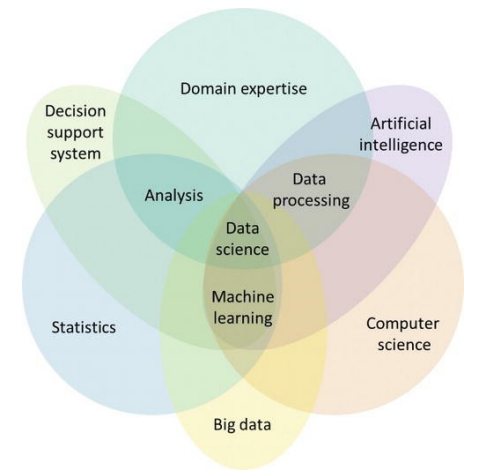
\includegraphics[scale=0.5]{images/Introduction/Intro1.png}
    \caption{Different part of machine learning and more}
\end{figure}

\textbf{Big Data} are data whose scale, diversity and complexity require new
architectures, techniques, algorithms and analytics to manage them and
extract value and hidden knowledge from.\\
Big data are generated by many sources like social media, sensors, devices,
and many others.

Those are characterized by the 5 V's:
\begin{itemize}
    \item \textbf{Volume}, as the name can say Big data work with
      incredible volume of data that exponentially increase over time.
    \item \textbf{Velocity}, there is some data that are generated at a
      high rate so we have to analyse them in real time.
    \item \textbf{Variety}, the data can come in various formats, types and
      structures like audio,video, text, \ldots
    \item \textbf{Veracity}, the data quality compromised by misrepresented
      , outliers, software bug and so on.
    \item \textbf{Value}, all the data has to be transform in something
      useful in decision making and to gain a business advantage.
\end{itemize}

\section{Data Science}
To use those data, they have to be analysed to extract information and
knowledge from them. This is the main goal of \textbf{Data Science}, that is a
field that tries to \textbf{extract knowledge} from data. It is a mix of

It takes the raw data, cleans them and applies Machine learning to create
models. The data can be generated or acquired and both have to be stored
in some infrastructure, file system or programming models. 

The data then has to be \textbf{pre-processed}, that is the first step in
data science, and it is divided into two parts: \textbf{data cleaning},
that is the process of detecting and correcting corrupt or inaccurate
records from a record set and \textbf{integration}, that is the process of
combining data from different sources to provide a unified view of them.

Then we have machine learning that is the process of fitting a model to 
data and then using that model to make predictions. The model is a 
mathematical representation of the data and it is used to make 
the predictions, but we will see more about this in the next chapters.

\begin{figure}[H]
    \centering
    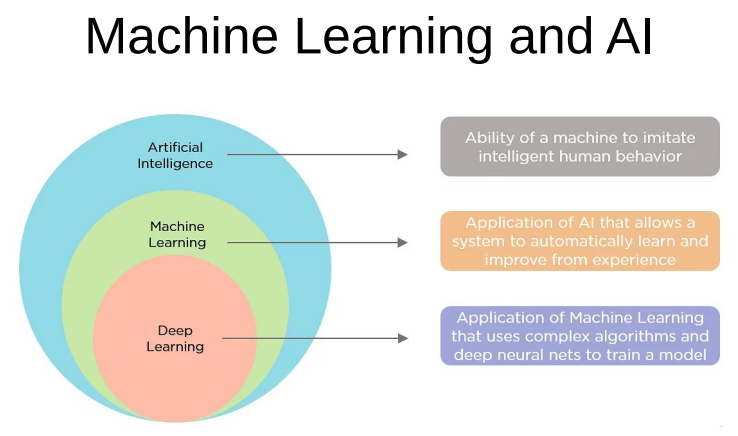
\includegraphics[scale=0.5]{images/Introduction/Intro2.png}
    \caption{Machine learning}
    \label{fig:enter-label}
\end{figure}

\chapter{Data Exploration Visualisation}\
\section{Theory}
A \textbf{Dataset} is a collection of data with a tabular representation includes rows and columns. The size of the dataset has a huge impact on the choice of the analyses, not always we can use certain algorithms because require considerable resources but there are solutions to reduce the size the cardinality preserving the completeness of the data.

Each column of the dataset represents on attribute or \textbf{feature} and every rows is a different sample, we can analyse attribute independently with their measurement, type and domain. To gain some information, starting from a theoretical distribution we use the min, max, avg, mean value, standard deviation or mathematical function.

To represent visual analyses for the univariate we use the histogram to show the distribution that can be classified as discrete probability function described by \textbf{probability mass function (PMF)} or continuous probability function described by \textbf{probability density function (PDF)}. But to be consistent and have better visualization we can't use the raw histogram so with the kernel density estimation (KDE) we can estimate continuous PDF based on samples
\begin{figure}[H]
    \centering
    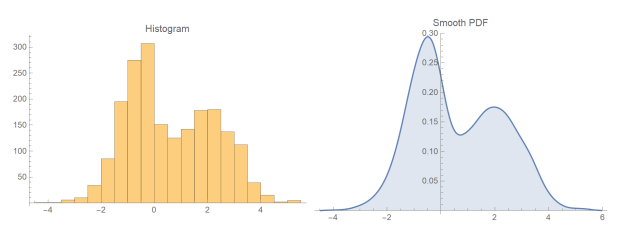
\includegraphics[scale=0.75]{images/DataExplVis/KernelDF.png}
    \caption{Caption}
    \label{fig:enter-label}
\end{figure}
To compute that we estimate f as the weighted average of neighboring observed data where the weight is defined by the kernel function, such that closer points are given higher weights and the estimated function is continuous and ‘smooth’.
\begin{center}
    $ f_{h}(x) = \frac{1}{m} \sum\limits_{i=1}^m K_{h} (x-x_{i})$
\end{center}

So KDE can produce a plot that is less cluttered and more interpretable but introduce some distortion on the data.

Cumulative distribution function (CDF) is needed to observe how the samples are distributed in different interval so to compute that we have to integrate the function from $ - \infty$ to $x$. This is very heavy in huge dataset so we can use Empirical Cumulative Distribution function (ECDF) that is an estimate of CDF that generates points in the sample. The ECDF is a step function that jumps up by 1/m at each of the m data points

\begin{figure}[H]
    \centering
    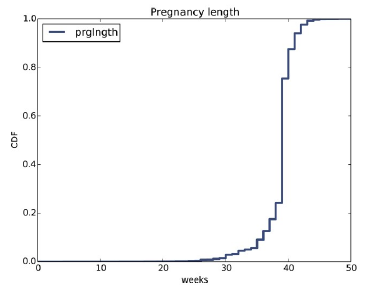
\includegraphics{images/DataExplVis/ECDF.png}
    \caption{Example of ECDF}
    \label{fig:enter-label}
\end{figure}

Percentiles indicates the value below which given percentage of observation in a group of observation falls and similarly there is the boxplot visualization. This 2 are standardized way of displaying the distribution data based on a summary values.
The boxplot can be a little tricky and this is the various part that composed it:
\begin{itemize}
    \item median: (Q2/50th Percentile): the middle value of the attribute.
    \item first quartile (Q1/25th Percentile): the middle number between the smallest number (not the “minimum”) and the median of the attribute.
    \item third quartile (Q3/75th Percentile): the middle value between the median and the highest value (not the “maximum”) of the attribute.
    \item interquartile range (IQR): 25th to the 75th percentile.
    \item whiskers (shown in blue)
    \item \textbf{outliers} (shown as green circles)
\end{itemize}

\begin{figure}[H]
    \begin{subfigure}{.5\textwidth}
        \centering
        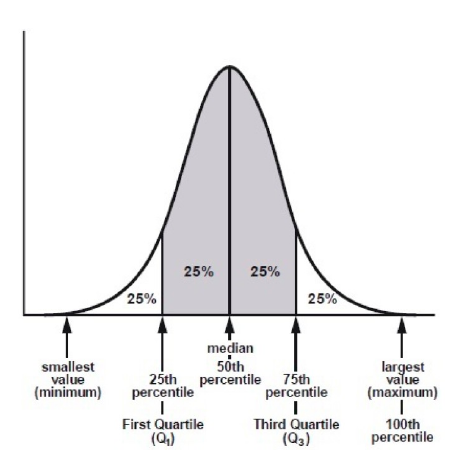
\includegraphics[width=.6\linewidth]{images/DataExplVis/Percentile.png}
        \caption{Percentile}
        \label{fig:sub1}
    \end{subfigure}
    \begin{subfigure}{.5 \textwidth}
        \centering
        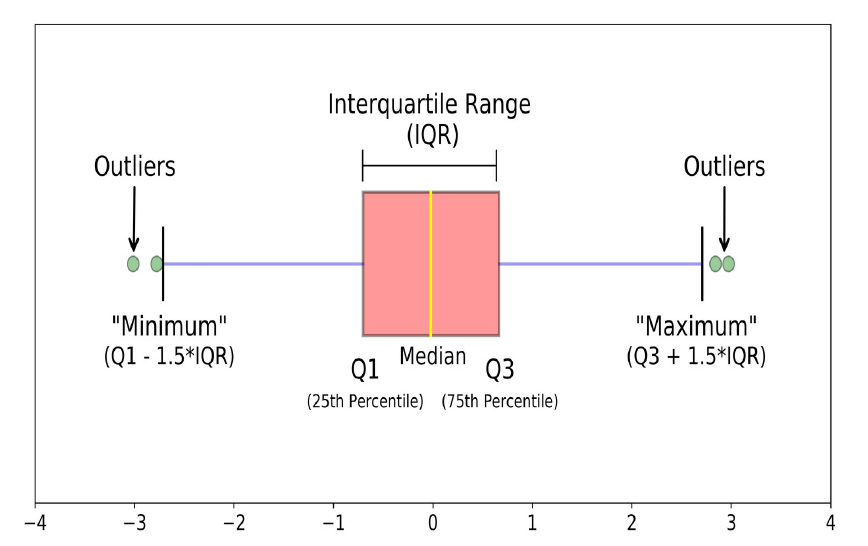
\includegraphics[width=.8\linewidth]{images/DataExplVis/Boxplot.png}
        \caption{Boxplot}
        \label{fig:sub1}
    \end{subfigure}
    \caption{Example of Percentile and Boxplot}
\end{figure}

The \textbf{Outliers} are extreme values that might be an errors in measurement and recording or an accurate reports of rare events. The best way to define/handle outliers depends on “domain knowledge” because it depends on what analysis you are planning to address.
Outlier can be detected by Generalized Extreme Studentized Deviate (GESD) but that can only be used in data set that follows a normal distribution. Another method to detect is DBSCAN that is based on a density clustering non-parametric algorithm.

However a dataset usually includes different features so the relationship between them have a key role to describe the entire dataset, this is called \textbf{correlation}. This is useful during the data exploration phase and to analyse specific data correlation because highly correlated features could be removed simplifying the performance of data driven algorithms

The simplest way to visually check for a relationship between 2 variables is a scatter plot, but to have a better comprehension  of the data we have to add some jitter or alpha parameters in order to retrieve density information

\begin{figure}[H]
    \begin{subfigure}{.5\textwidth}
        \centering
        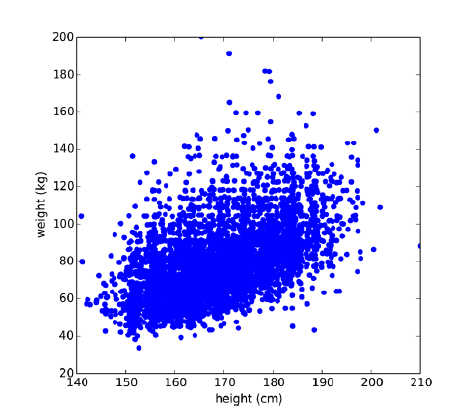
\includegraphics[width=.6\linewidth]{images/DataExplVis/Scatter1.png}
        \caption{Scatter with jitter}
        \label{fig:sub1}
    \end{subfigure}
    \begin{subfigure}{.5 \textwidth}
        \centering
        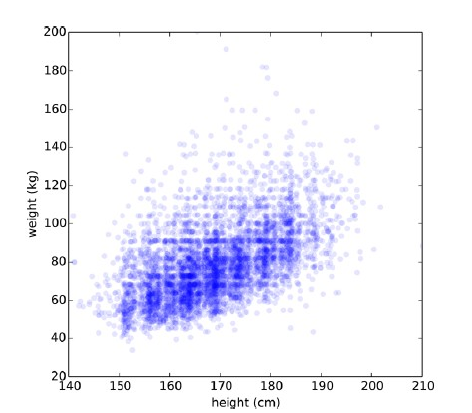
\includegraphics[width=.6\linewidth]{images/DataExplVis/Scatter2.png}
        \caption{Scatter with transparency}
        \label{fig:sub1}
    \end{subfigure}
    \caption{Example of Scatterplot}
\end{figure}

Moreover we can use scatterplot percentiles with every line that represents one percentile to focus on the main data and not the outlier.

A \textbf{correlation} is a statistic intended to quantify the strength of the relationship between two variables. Possible way to compute correlations are:
\begin{itemize}
    \item Covariance: is a measure of the joint variability of two random variables. In order to compare two variables, they must have the same unit of measurement or normalized
    \item Pearson: Solves the problem of normalization but can only detects linear correlation
    \item Spearman
\end{itemize}
The formulas for the correlation are:
\begin{center}
    $corr(x,y)=  \dfrac{covariance(x,y)}{sd(x) * sd(y)}  $\\
    $covariance(x,y) = \dfrac{1}{n-1} \sum\limits_{k=1}^n (x_{k} - \overline{x} )(y_{k} - \overline{y} )$\\
    $standard\_deviation(x)= sd(x)= \sigma(x)= \sqrt{\dfrac{1}{n-1} \sum\limits_{k=1}^n (x_{k} - \overline{x} )^2 } $\\
    $standard\_deviation(y)= sd(x)= \sigma(y)= \sqrt{\dfrac{1}{n-1} \sum\limits_{k=1}^n (y_{k} - \overline{y} )^2 } $\\
    $ \overline{x}$ and $\overline{y} $ are the mean of all x and y samples calculated with $\overline{x} = \dfrac{1}{n} \sum\limits_{k=1}^n  x_{k} $
\end{center}
Pearson is only for linear correlation and have result between {-1;1} and we use Spearman's Rank Correlation, that assesses how the relationship between two variables can be transformed into  a rank and can be described using a monotonic function and the advantage is that in some cases the Spearman index allows to find a correlation when the Pearson index returns a value close to 0.
The formulas changes to:
\begin{center}
    $ r_s =  \rho_{(R(x),R(y))} = \dfrac{cov(R(x),R(y))}{\sigma_{R(x)} \sigma_{R(y)}}$\\
    if all m ranks are distinct we can use $ r_s = 1 - \dfrac{6 \sum (R(X_i) - R(Y_i))^2}{m(m^2 -1)}$
\end{center}
Other data visualization are:
\begin{itemize}
    \item heatmap
    \item Word Cloud
    \item PCA
    \item T-SNE
\end{itemize}

    




\chapter{Data Pre Processing}
The data usually have a lot of quality issues due to thing like noise
or outliers, missing values or duplicate data. One would like to have
a clean data set to work with, but this is not always the case.  The
The action to perform to \textit{prepare} the data is called the
\textbf{data cleaning}

\section{Similarity and Dissimilarity}
\begin{boxH}
  We can define the \textbf{similarity}, or \textbf{dissimilarity},
  between two data object as a numerical measure of how alike or
  different they are.
\end{boxH}
One of the most common similarity measure is the \textbf{distance} 
between two objects, and there are a lot of different distance
measures.

\subsection{Euclidean Distance}
The \textbf{euclidean distance} is the simplest one, which can be
defined as the square root of the sum of the squared differences
between the two objects. It is defined as:
\begin{equation}
  d(x,y) = \sqrt{\sum\limits_{k=1}^n (x_k - y_k)^2 }
\end{equation}
where $x$ and $y$ are two objects, and $x_k$ and $y_k$ are the $k$-th
attributes of the two objects.

Standardizing of the data may be needed to avoid that some attributes
dominate the distance measure.

\subsection{Minkowsky Distance}
\textbf{Minkowsky distance} is a generalization of Euclidean Distance,
and it is defined as:

\begin{equation}
  d(x,y) = (\sum\limits_{k=1}^n | x_k - y_k |^r )^{1/r} 
\end{equation}
where $r$ is a parameter that can be set to 1, 2 or $\infty$.
If $r=1$ we have the \textbf{Manhattan} distance, if $r=2$ we have the 
\textbf{Euclidean} distance, and if $r=\infty$ we have the 
\textbf{Chebyshev} distance.

\subsection{Mahalanobis Distance}
\textbf{Mahalanobis distance} measures the distance between two points
with respect to a probability distribution with covariance matrix $S$
and also  is thus unit less, scale-invariant, and takes into account
the correlations of the data set. It is defined as:
\begin{equation}
  d(x,y,S) = \sqrt{(x-y)^T S^{-1} (x-y)}
\end{equation}

\section{Data pre-processing tasks}
Data pre-processing has many different tasks that have to be carried
out in order to have a clean data set to work with. We will go over
the main ones.
\subsection{Data aggregation}
\begin{boxH}
  \textbf{Data aggregation }is the process of \textbf{combining} two
  or more \textbf{attributes}(or objects) into a single attribute(or
  object).
\end{boxH}
This is done for three main reasons:
\begin{itemize}
  \item To reduce the number of attributes or objects(Data reduction)
  \item To change the scale of the data, for example from daily to
    monthly
  \item To \textit{stabilize} the data, for example by taking the
    average of the data to reduce the variance
\end{itemize}
Here's an example of data aggregation:
\begin{figure}[H]
  \centering
  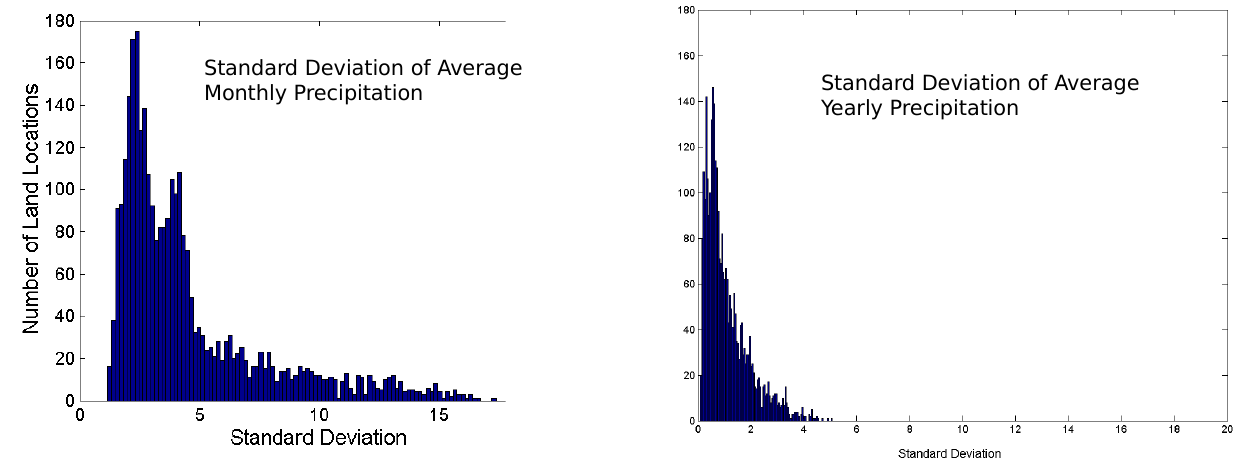
\includegraphics[scale=0.4]{images/Data
  pre-process/precipitation aggregation.png}
  \caption{Example of data aggregation}
  \label{fig:data-aggregation}
\end{figure}
as you can see from figure \ref{fig:data-aggregation}, the yearly
precipitation has much less variability then the average monthly
one.
\subsection{Data reduction}
The main goal of data reduction is to generate a reduced
representation of the dataset, with a much smaller volume but 
still able to produce the same or similar analytical results.\\
This can be done trough different techniques.
\subsubsection{Sampling}
\textbf{Sampling} is the \textbf{main technique} employed for data selection
and it is often used for both the preliminary investigation of the
data and the final data analysis because processing the entire set of
data of interest might be too expensive or time consuming.\\
The key principle for effective sampling is the following: a good
sample will always work like the dataset and can approximately have
the same property.\\
There are several types of sampling like the simple random sampling or
the stratified one that split the data into several partition and then
draw samples from each partition.

\begin{figure}[H]
  \centering
  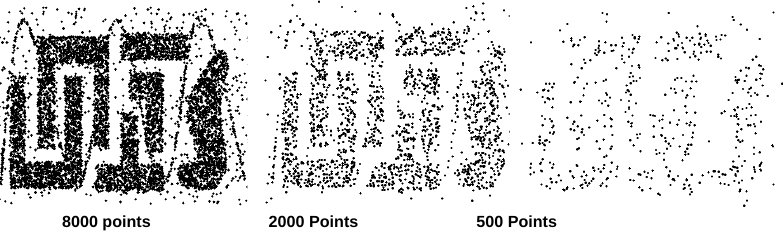
\includegraphics[scale=0.5]{images/Data
  pre-process/sampling.png}
  \caption{Example of sampling}
  \label{fig:sampling}
\end{figure}
There are two main types of sampling:
\begin{itemize}
  \item \textbf{Simple random sampling}: each object has the same probability
    of being selected. Of this type two main methods are: 
    \begin{itemize}
      \item \textbf{With replacement}: the same object can be selected
        more than once because its not removed from the population
      \item \textbf{Without replacement}: the same object can be selected
        only once because it is removed from the population
    \end{itemize}
  \item \textbf{Stratified sampling}: the population is divided into
    subpopulations, and the right number of objects is sampled from
    each subpopulation
\end{itemize}

\subsubsection{Curse of Dimensionality}
When feature dimensionality increases, data becomes increasingly
sparse in the space that it occupies and the definitions of density
and distance between points, which is critical for clustering and
outlier detection, become less meaningful.\\
This is the \textbf{curse of dimensionality}, and it is a common 
problem in data mining and machine learning.
\subsubsection{Feature Subset Selection}
This is another way to reduce the dimensionality of the data, and it
is the process of identifying and removing as much of the irrelevant 
and redundant information as possible.\\
A feature is considered \textbf{irrelevant} if it does not hold any
useful information for the data mining task at hand, while a feature
is considered \textbf{redundant} if it holds the same information as 
another feature.
\subsubsection{Recursive feature elimination}
One method is called recursive feature elimination that assigns
weights to features and then selects features by recursively 
considering smaller and smaller sets of features.  First, the 
estimator is trained on the initial set of features and the 
importance of each feature is obtained, the least important features 
are pruned from current set of features. That procedure is 
recursively repeated on the pruned set until the desired number of 
features to select is eventually reached.
\section{Feature Engineering}
\begin{boxH}
  A \textbf{feature} is an individual measurable property or
  characteristic of the raw data. \textbf{Feature engineering} is the 
  act of extracting features from raw data and transforming them to 
  more useful, from a lot to few.
\end{boxH}
Usually formats that are suitable for machine learning are used.
According to the type of data under analysis different feature
engineering techniques are needed:
\begin{itemize}
  \item \textbf{structured data}: data that can be easily organized
    into a table format, like a spreadsheet
  \item \textbf{unstructured data}: data that does not have a 
    pre-defined format, like text
\end{itemize}
There are many diffrent techniques for feature engineering, like
normalization, discretization, binarization, and many others.

\subsection{Data Transformation}
\textbf{Data transformation} is the process of converting data from
one format to another and it is useful because non numerical data is
difficult to analyze if not transformed into numerical and to capture
important information or to better visualize the data

\subsection{Discretization}
\textbf{Discretization }is the process of converting a continuous
attribute into an ordinal attribute: A potentially infinite number of
values are mapped into a small number of categories, for example
{high, medium, low} or binary attributes or one-hot encoding. 

\subsection{Binarization}
\textbf{Binarization} is the process of converting numerical data into 
binary data, for example by setting a threshold value and converting 
all values above the threshold to 1 and all values below the threshold 
to 0.\\
Binarization can be even performed on continuous attributes, by
firstly mapping them in a categorical one(eg. heigh measured as
\{low,medium,high\} and then binarizing them trough one-hot encoding.
\subsubsection{One-hot encoding}
\textbf{One-hot encoding} is a data representation method that
converts categorical data into a binary matrix, where each category
is represented by a binary vector.\\
Each bit represents a category, and the bit is set to 1 if the 
category is present and 0 otherwise.
\begin{figure}[h]
  \centering
  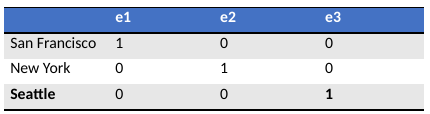
\includegraphics[scale=0.6]{images/Data
  pre-process/one hot encoding.png}
  \caption{Example of one-hot encoding}
  \label{fig:one-hot-encoding}
\end{figure}
Take a look at figure \ref{fig:one-hot-encoding} to see an example of 
one-hot encoding, as you can see the attribute city can only assume 3
values.

\subsubsection{Dummy Coding}
One-hot encoding allows for k degrees of freedom( where k is the
number of categories), but variable itself needs only k–1 degrees of 
freedom.\\
Dummy Coding encodes the effect of each category relative to the
reference category encoded with zeroes (Seattle).
\begin{figure}[H]
  \centering
  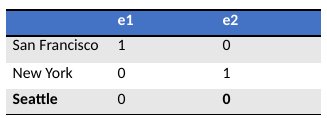
\includegraphics[scale=0.6]{images/Data
  pre-process/dummy coding.png}
  \caption{Example of dummy coding}
  \label{fig:dummy-coding}
\end{figure}

\subsubsection{Effect Coding}
Effect coding is similar to dummy coding, but the reference category 
is encoded with -1 instead of 0.\\ 
Effect coding is useful when you want to compare each category to the 
average of all categories.

\begin{figure}[H]
  \centering
  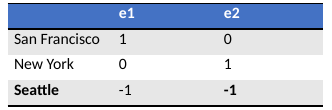
\includegraphics[scale=0.6]{images/Data
  pre-process/effect coding.png}
  \caption{Example of effect coding}
  \label{fig:effect-coding}
\end{figure}

\begin{figure}[H]
  \centering
  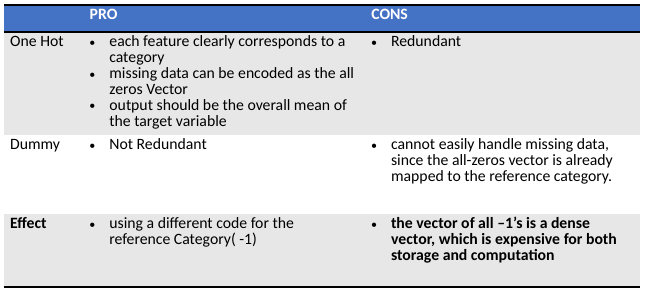
\includegraphics[scale=0.6]{images/Data
  pre-process/coding comparison.png}
  \caption{Comparison between dummy, effect and one-hot coding}
\end{figure}

\section{Attribute Transformation}
An \textbf{attribute transformation} is a mapping of the entire set of
values of a given attribute to a new set of replacement values such 
that each old value can be identified with one of the new values.\\ 
If can be a simple function like $x' = x^2$ or a more complex one like 
$ x' = \dfrac{x-\mu}{\sigma}$


\subsection{Normalization}

\textbf{Normalization} refers to various techniques to adjust to
differences among attributes in terms of mean, variance, range. It is
performed with the attribute transform that is is a function that maps
the entire set of values of a given attribute to a new set of
replacement values such that each old value can be identified with one
of the new values. There are a lot of different normalization.
\subsubsection{Min-Max normalization}
\begin{center}
    Min-max normalization  $x'= \dfrac{x-x_{min}}{x_{max} - x_{min}}$
\end{center}
Min Max-normalization rescales the functions and is a unity based
normalization, is a technique that bring all values into the range of
[0,1] retains the shape of the distribution, as shown in the figure 
\ref{fig:min-max-normalization}.
\begin{figure}[H]
    \centering
    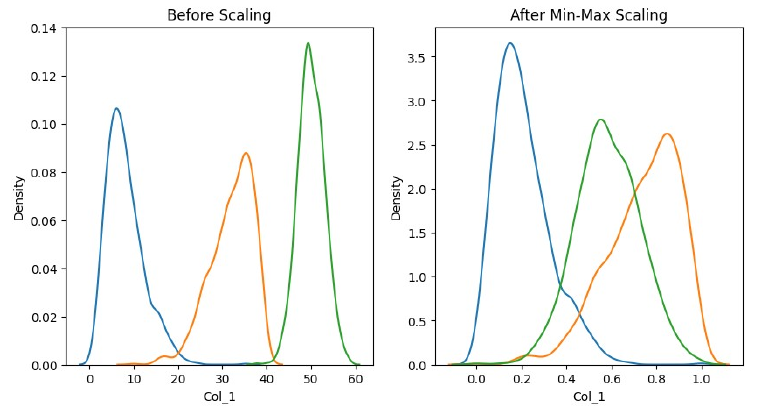
\includegraphics[scale=0.5]{images/Data pre-process/MINMAX.png}
    \caption{Example of Min max normalization}
    \label{fig:min-max-normalization}
\end{figure}
\subsubsection{Standardization}

\begin{center}
    Standardization  $x'= \dfrac{x- \mu}{\sigma}$
\end{center}

Standardization is another kind of normalization ans is a bit
different from the previous one because it is not bounded to a certain
range and it's used when we want to ensure zero mean and
unit standard deviation.
\begin{figure}[H]
    \centering
    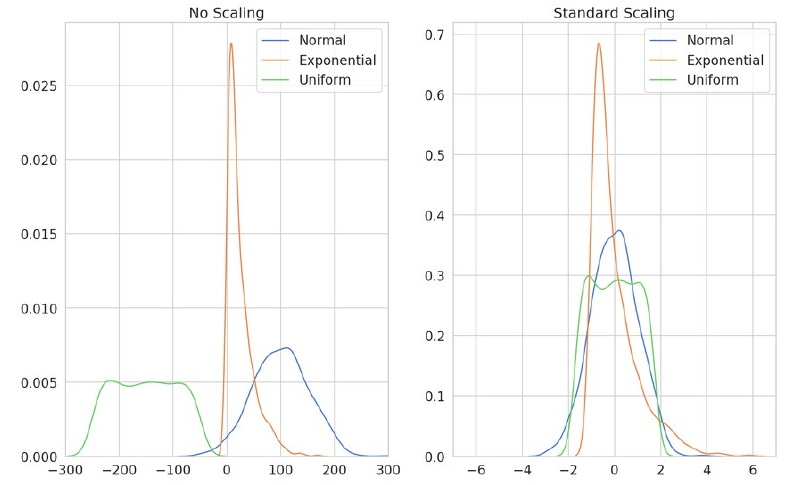
\includegraphics[scale=0.5]{images/Data pre-process/Standard.png}
    \caption{Example of standardization}
    \label{fig:enter-label}
\end{figure}

\section{Data preparation for document data}

Document may be modeled in different ways and the choice heavily
affects the quality of the mining result: often document are
represented as a set of features and might represent set of
characters, word, term, concept. 
\begin{boxH}
  Document preprocessing is the activity of generating a structured
  data representation of document data.
\end{boxH}
This includes 5 main steps:
\begin{enumerate}
    \item Document splitting
    \item Tokenization
    \item Case normalization
    \item Stopword removal
    \item Stemming
\end{enumerate}
\subsection{Document splitting}
Document splitting is based on the data analytics goal, documents can
be split into sentences, paragraphs, or analyzed in their entire
content.\\
Short documents are typically not split, like emails or social posts
but long documents can be split into paragraphs or sentences, or even
analyzed as a whole.
\subsection{Tokenization}
Tokenization is the process of breaking text into words, phrases, 
symbols or other meaningful elements.\\
To perform tokenization, one must first identify the boundaries of 
sentences based on punctuation and capitalization, and then split the 
text into words.
\subsection{Case normalization}
This step converts each token to completely upper-case or lower-case
characters.\\
Capitalisation helps human readers differentiate, for example, between
nouns and proper nouns and can be useful for automated algorithms as
well. However, an upper-case word at the beginning of the sentence
should be treated no differently than the same word in lower case
appearing elsewhere in a document.
\subsection{Stopword removal}
“Stop words” refers to the most common words in a language, for
example propositions, articles, and conjunctions.\\
Those are usually filtered out before or after processing of text,
because most likely they have little semantic meaning.
\section{Text representation}
Some algorithms can't process raw textual data directly, so documents
are converted into feature vectors for easier handling. A feature is a
simple entity, representing a dimension in the feature space, and a
document is represented as a vector of features with their
corresponding weights.
\subsection{Bag of words}

\textbf{Bag of words} are the representation for the words in a
document where every word is considered as a feature, where the
dimension is equal to the number of different words and there is a set
of weights, one for each distinct word.

\begin{figure}[H]
    \centering
    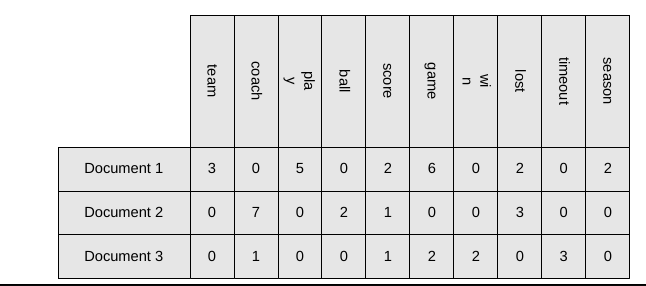
\includegraphics[scale=0.6]{images/Data pre-process/Word-bag.png}
    \caption{Example of bag of word}
    \label{fig:enter-label}
\end{figure}

\subsection{Weighting schemes}
Weighting schemes are used to assign weights to the words in the
document. They can be:
\begin{itemize}
    \item  Binary
        \begin{itemize}
            \item One, if the corresponding word is present in the document
            \item Zero, otherwise
            \item Occurrences of all words have the same importance
        \end{itemize}
    \item Simple document frequency
        \begin{itemize}
            \item The number of times in which the corresponding word occurs in the document
            \item Most frequent words are not always representative of the document content
        \end{itemize}
    \item Term frequency inverse document frequency (tf-idf)
        \begin{itemize}
            \item Tf-idf of term $t$ in document d of collection $D$ (consisting of m documents)
            \item Terms occurring frequently in a single document but rarely in the whole collection are preferred
            \item  tf-idf(t)$=   freq(t,d)\cdot log(\dfrac{m}{freq(t,D)} ) $
        \end{itemize}
\end{itemize}
Notice that the tf-idf is the most used weighting scheme because it 
gives more importance to the words that are more relevant to the 
document, and is also most suitable for a single document consisting
of many sections or subsections or a collection of documents.


 

\chapter{Dimensionality reduction}
\section{PCA}

It is obvious that less significant feature are better than a lot of irrelevant feature and also there is a problem of visualization with multivariate data. Moreover it is difficult to extract useful information from multivariate data.
So the problem of dimensionality reduction is about learn hypothesis map that reads representation of data point and transforms it to a set of features, the advantage are:
\begin{itemize}
    \item Capture the important information in a data set more efficiently than the original attributes
    \item Allow data to be more easily visualized
    \item Reduce overfitting
    \item Avoid curse of dimensionality
    \item Reduce amount of time and memory required by algorithms
    \item Help to eliminate irrelevant features or reduce noise
\end{itemize}

It was firstly introduced by y Pearson (1901) and Hotelling (1933) to describe the variation in a set of multivariate data in terms of a set of uncorrelated variables. The goal is reduce the feature, so starting from $n$ features we want to have $p$ new feature where $p$ << $n$ keeping more information as possible with the p variable that will be \textbf{uncorrelated}.

\begin{figure}[H]
    \centering
    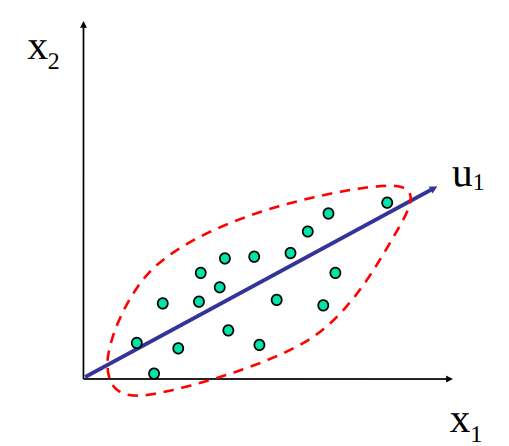
\includegraphics[scale=0.65]{images/DimRed/PCA1.png}
    \caption{Example of PCA}
    \label{fig:PCA}
\end{figure}

For example in the figure before we have in green the point with the feature $x_{1}$ and $x_{2}$ and we construct a function called $u_{1}$ to summarize this 2 features into 1; if we have bigger data we can choose between different $u$, but in this case the function have to be the one with the \textbf{largest variation}.

\begin{figure}[H]
    \centering
    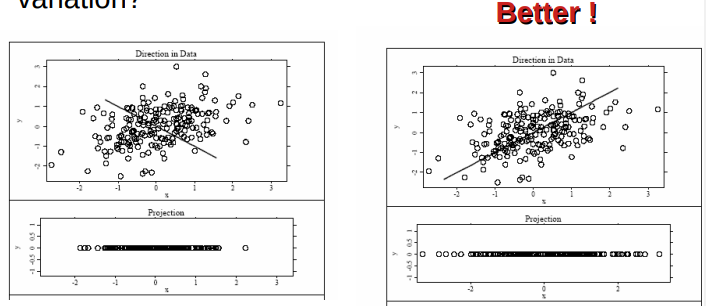
\includegraphics[scale=0.7]{images/DimRed/PCA2.png}
    \caption{Example of choosing the correct function $u$}
    \label{fig:enter-label}
\end{figure}

Principal component analysis is useful if there is some redundancy in variables or the data do not ‘span’ the whole of n dimensional space, because of this redundancy or space not covered, it is possible to
reduce the observed variables into a smaller number of principal components (artificial variables) 

It can be viewed as a rotation of the existing axes to new positions in the space defined by original variables and this new axes are orthogonal and represent the directions with maximum variability.
\begin{figure}[H]
    \centering
    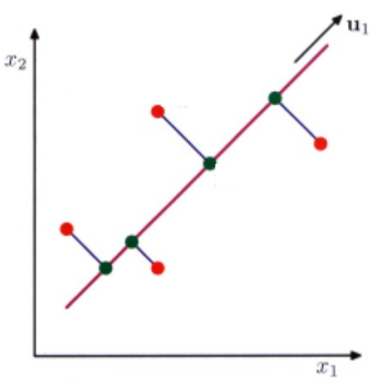
\includegraphics[scale=0.5]{images/DimRed/PCA3.png}
    \caption{PCA maximization}
    \label{fig:enter-label}
\end{figure}
\emph{\textbf{Definition}}: Principal component analysis seeks a space of lower dimensionality, known as the principal subspace and denoted by the magenta line, such that the orthogonal projection of the data points (red dots) onto this subspace \textbf{maximizes the variance of the projected points} (green dots). An alternative definition of PCA is based on \textbf{minimizing the sum-of-squares of the projection errors}, indicated by the blue lines.


A principal component can be defined as a linear combination of optimally-weighted observed variables and The number of components that can be extracted in a principal component analysis is equal to the number of observed variables. Oftenn only the first few components account for meaningful amounts of variance $(p<n)$. When the analysis is complete, the resulting components will display varying degrees of correlation with the observed variables, but are \textbf{completely uncorrelated} with one another

\subsection{Math part}
\paragraph{Single attribute}
With a single feature the calculus of the variance is very simple because the variance is only the power of 2 of the standard deviation
\begin{center}
    $variance = sd^2$\\
    $sd = \sqrt{\dfrac{1}{m-1} \sum\limits_{i=1}^m (x_i - \overline{x})^2}$ \\
    $s^2 = \dfrac{1}{m-1} \sum\limits_{i=1}^m (x_i - \overline{x})^2$
\end{center}
\paragraph{Two attributes}
Covariance: measures the correlation between x and y
\begin{center}
    $cov(x,y) = \dfrac{1}{m-1} \sum\limits_{i=1}^m (x_i - \overline{x}) (y_i - \overline{y})$
\end{center}
\begin{itemize}
    \item cov(x,y)=0: independent, we want to reach that
    \item cov(x,y)>0: move same direction
    \item cov(x,y)<0: move opposite directions
\end{itemize}
\paragraph{More than two attributes}
To have all the other number of feature we can create a covariance matrix like in the next figure, that matrix contains covariance values between all possible dimensions.
\begin{figure}[H]
    \centering
    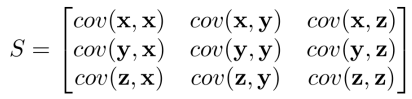
\includegraphics{images/DimRed/PCA4.png}
    \caption{Example of covariance matrix}
    \label{fig:enter-label}
\end{figure}

\begin{center}
    Sample covariance matrix S (n x n) of X (m x n) can be written as:\\
    $ S = \dfrac{1}{m-1} \sum\limits_{i=1}^m (X - \overline{X})^t (X - \overline{X})$\\
    where $\overline{X}$ (m x n) is the matrix of the mean attributes (all m rows are equal, corresponding to the mean of all m rows of X)
\end{center}
Before proceeding with something useful for the PCA there are some mathematical stuff to know.
\paragraph{Eigenvalues and eigenvector}
Vectors u having same direction as Au are called eigenvectors of A (A is an n by n matrix),  In the equation Au=$\lambda$u, $\lambda$ is called an eigenvalue of A.\\
$\begin{bmatrix}
    2 & 3 \\
    2 & 1 
\end{bmatrix}
=
\begin{bmatrix}
    3\\
    2
\end{bmatrix}
= 4
\begin{bmatrix}
    3\\
    2
\end{bmatrix}
$\\\\
Then we can look to some matrix formulas:
\begin{center}
    $(A^t)^t =A $\\
    $P^{-1} = P^t$\\
    $(A \pm B) =A^t \pm B^t$\\  
    $(cA)^t =cA^t$\\
    $(AB)^t= B^t A^t$
\end{center}

Now we can start talking about the orthogonality and orthonormality. 
Two vectors $u_1$ and $u_2$ (n x 1) for which $u_1^t u_2=0$ holds are said to be orthogonal, the idea is that to be orthogonal in the image they have to be perpendicular.
The feature transformation is a change of the basis with orthonormal vectors so we have to find orthonormal P (n x n) such that $X'= XP^t$ with cov(X') diagonalized (\textbf{variables uncorrelated}). The (first p) rows of P are the principal components of X.
 
To find P with cov(X') diagonalized (diagonal equal to 0):
\begin{center}
    $ cov(X') = \dfrac{1}{m-1} (X')^t (X')$  if X' has zero means so we can just cancel $\overline{X}$\\
    = $\frac{1}{m-1} (X P^t)^t (XP^t)$ \\
    = $\frac{1}{m-1} X^t P X P^t $ = $\frac{1}{m-1} P(X^t X )P^t $ = $\frac{1}{m-1} PAP^t$
\end{center}

That $A =X^t X$ is symmetric (n x n), therefore there is a matrix E of eigenvectors of A and a diagonal Matrix called D such that $A = EDE^t$. Now we define P to be the transpose of the matrix E of eigenvectors $P:= E^t$ then we can write A as $ A = P^t D P $. Remember that $E = (u_1, u_2, u_3, \dots)$ as column, all the possible eigenvectors.

With this definition we substitute the values:
\begin{center}
    $ cov(X') = \dfrac{1}{m-1} PAP^t = \dfrac{1}{m-1} PP^t D PP^t= \dfrac{1}{m-1}D =S'$
\end{center}

If we define P as the transpose eigenvector matrix will have as a result a Diagonal (D) covariance matrix with the diagonal equal to 1 and 0 in any other.

$S' = cov(X') =
\begin{bmatrix}
    1 & 0 & 0 \\
    0 & 1 & 0 \\
    0 & 0 & 1 \\
\end{bmatrix}$

P diagonalized cov(X') where P is the transpose of the matrix of eigenvectors of $ A=XX^t$ and the principal components  of X are the eigenvectors of $A=X^tX$, moreover the $i_{th} $ diagonal value of cov(X') is the variance of X' along $u_i$ (along the $i_{th}$ principal component, the $i_{th}$ row of P).

$S' = \begin{bmatrix}
    \sigma_1 & 0 & 0 \\
    0 & \sigma_2 & 0 \\
    0 & 0 & \sigma_3 \\
\end{bmatrix}
    \\
    \sigma_1 = cov(x_1,x_1) = var(x_1)
$

Essentially, we need  to take the covariance`matrix of the original matrix X and compute:
\begin{enumerate}
    \item Eigenvalues: explained variance
    \item Eigenvectors: new axis, principal components
\end{enumerate}

In the diagonal matrix we have to take the maximum eigenvalues, that has the maximum variance, and it will be the first component or Principal Component PC1. The second, instead, have the direction with maximum variation left in data orthogonal to PC1. The eigenvector corresponding to the second largest eigenvalue.

\subsubsection{Steps of PCA}
\begin{enumerate}
    \item Let $\overline{X} $ be the mean matrix (all rows are equal, corresponding to the mean of all rows)
    \item Adjust the original data by the mean $X-\overline{X}$
    \item Compute the covariance matrix S of X: $ S = \dfrac{1}{m-1} \sum\limits_{i=1}^m (X - \overline{X})^t (X - \overline{X})$
    \item Find the eigenvectors and eigenvalues of S
    \item For matrix S, vectors u (=column vector) having same direction as Su, with factor $\lambda$
    \item Eigenvalues $\lambda_i$ corresponds to variance on each component i=1,...,n
    \item Thus, sort by $\lambda_i$
    \item Take the first p eigenvectors $u_i$; where p is the number of top eigenvalues. Form matrix P
    \item These are the directions with the largest variance
    \item Project the original data: $XP^t$
\end{enumerate}

There is a correlation between Eigenvalues and the Variance because Eigenvalues $\lambda_i$ are used for calculation of [\% of total variance] (Vi) for each component i: $ V_i = 100 \dfrac{\lambda_i}{\sum\limits_{j=1}^n \lambda_j} $ and if the data are \textbf{standardized} $\sum\limits_{j=1}^n \lambda_j = n $

\begin{figure}[H]
    \begin{subfigure}{.4\textwidth}
        \centering
        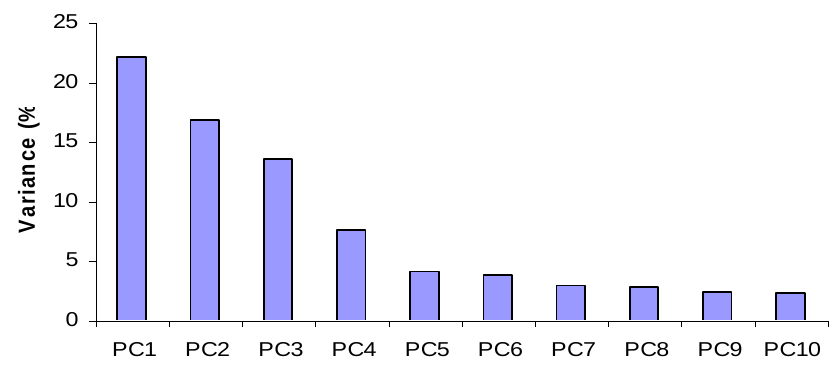
\includegraphics[width=1\linewidth]{images/DimRed/PCA5.png}
        \caption{Visual representation of Variance}
        \label{fig:sub1}
    \end{subfigure}
    \begin{subfigure}{.5 \textwidth}
        \centering
        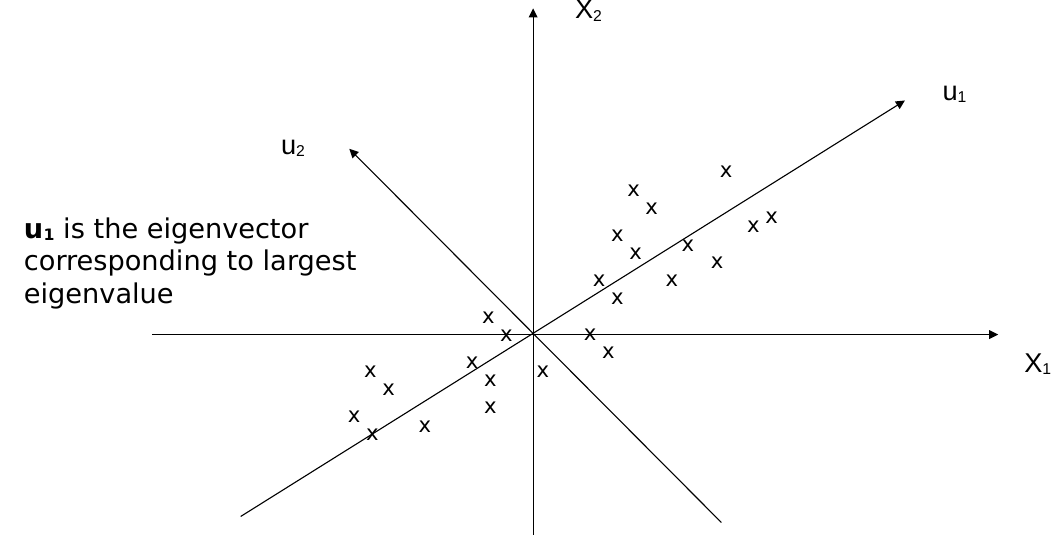
\includegraphics[width=1\linewidth]{images/DimRed/PCA6.png}
        \caption{New basis with $u_1$ and $ u_2$}
        \label{fig:sub1}
    \end{subfigure}
    \caption{Eigenvalues and Eigenvectors}
\end{figure}

\subsubsection{Properties}
 The properties of the principal components are:
 \begin{itemize}
     \item  linear combinations of the original variables
     \item  uncorrelated with each other
     \item capture as much of the original variance as possible
 \end{itemize}

Another important things to considered is the criteria of when to stop the PCA (choosing the p).
\begin{enumerate}
    \item Kaiser criterion: keep PCs with eigenvalues > 1 (variance explained more than a single original variable)
    \item Proportion of variance explained: enough PCs to have cumulative variance explained that is larger than a threshold (e.g., 66\%)
    \item  Elbow method: start of the bend in the line (point of inflexion) indicate how many components are retained
\end{enumerate}
\begin{figure}[H]
    \centering
    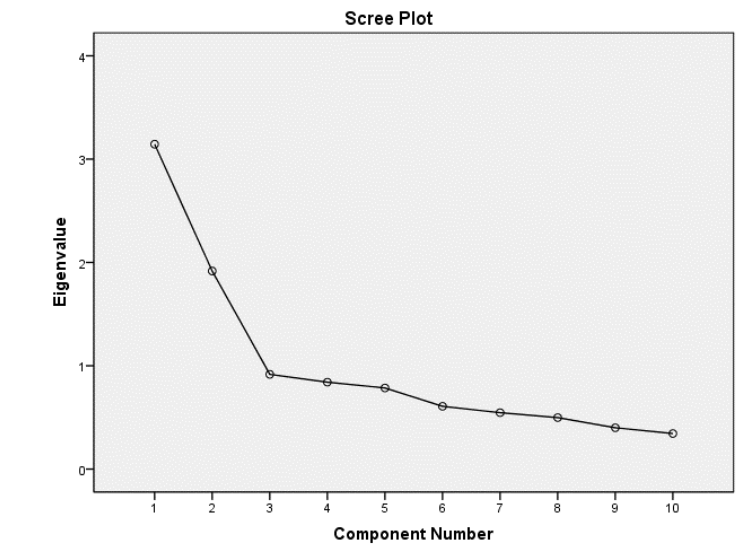
\includegraphics[scale=0.5]{images/DimRed/PCA7.png}
    \caption{Example of PCA Elbow method}
    \label{fig:enter-label}
\end{figure}

\subsection{Proof of eigenvalues - maximize variance}
Assuming $X \in R^{m \times n}$ as the data and $x_{i,j}$ as one value.
We want to find a number of feature $p << n$ that describe the entire data in an efficient way (best variance possible). In the example with $p=1$ we want to have only one feature and 1 vector and trying to maximize the variance. 
So the vector called $u_1 \in R^{1 \times n}$. The projection on the data has to be $ x_i \times u_1^T$ on a single dimension.\\
It is time to calculate the \textbf{mean projected data} as $ \overline{x} \times u_1^T $ and then the variance $ \frac{1}{m-1} \sum\limits_{i=1}^m (x_i \times u_1^T - \overline{x} \times u_1^T)^2$. The aim is to maximize this function.\\

max $ \frac{1}{m-1} \sum\limits_{i=1}^m (x_i \times u_1^T - \overline{x} \times u_1^T)^2$ =  max $(u_1 S u_1^T)$ with S equal to the covariance of the original matrix, but max $(u_1 S u_1^T)$ derivative tend to infinite because $|| u_1||$ tend to infinite. We add the constraint $|| u_1||$ that allows $u_1 u_1^T =1$.\\
$max_{u_1} (u_1 S u_1^T + \lambda (1 - u_1 u_1^T  ) $ with the second part that is a penalty to not consider the constrain. We do the derivative of that function in respect of $u_1$ as $ 2 S U_1^T - \lambda 2u_1^T = 0 $. NB = 0 because it is the results we want in order to maximize.\\
We obtain $S u_1^T = \lambda u_1^T $ that is the eigenvalue and eigenvector formula with $u_1$ eigenvector and $\lambda$ eigenvalue. Left multiplying by $u_1$ we obtain $u_1 S u_1^T = u_1 \lambda u_1^T $ and then we can change $u_1 \lambda u_1^T \rightarrow \lambda u_1 u_1^T$ , since $ u_1 u_1^T = 1$ we finally have $u_1 S u_1^T = \lambda$.

So in the left we have the variance of the projected data. So to maximize the variance we have to choose the maximum eigenvalue.




\section{Non linear dimensionality reduction}
Not all the data are linear so PCA don't work on all possibility.
\textbf{Kernel PCA} transform points on different feature space and then apply PCA and the results are not in a linear space.
\textbf{T-SNE} frequently used only for visualization, function with probability distribution on n-dimensional space and thern we take a similar probability distribution on lower p-dimensional space. This have to be performed iteratively until the Kullback-Leibler divergence between  distribution is minimized.
\chapter{3 Component}
The three components of Machine learning are \textbf{model,data and loss}, all is a combination of this 3 components in different way.

\section{Data}
Data are a set or a collection of data point and the data points could be objects, records, cases, samples, entities, or instances that carries information called feature or label.
Features are low-level properties easy to measure or compute instead labels are high level quantity of interest difficult to measure or determine. They need to be in good number because we should use only most relevant features but not fewer, and missing some relevant feature is really bad for accuracy. Also use irrelevant features waste computational power and might cause overfitting.

Label is \textbf{design choice} because you choose the label of a data point, by choosing label you define the ML problem or learning task. The labels could be categorical or numerical, for the first we can choose also between Binary or multi class classification instead for the numerical we have a regression task
\begin{figure}[H]
    \centering
    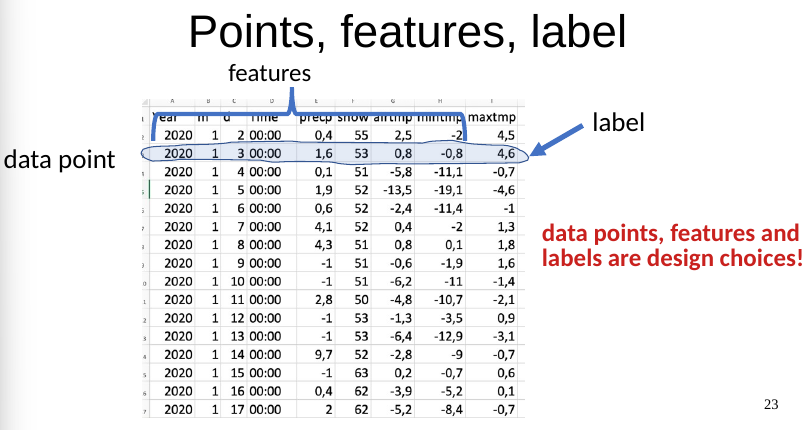
\includegraphics[scale=0.4]{images/3Comp/3Comp1.png}
    \caption{Example of tabular Data}
    \label{fig:enter-label}
\end{figure}
The feature can be seen as a matrix: \\
$ X = (x^{(1)} , x^{(2)}, \dots , x_{(m)})^t = \begin{bmatrix}
    x_1^{(1)} & x_2^{(1)} & \dots & x_n^{(1)} \\
    x_1^{(2)} & x_2^{(2)} & \dots & x_n^{(2)} \\
    \vdots & \vdots & \ddots & \vdots \\
    x_1^{(m)} & x_2^{(m)}& \dots &x_n^{(m)}
\end{bmatrix}
$\\
The labels as $y = (y_1, y_2,\dots, y_3 ) \in \mathbb{R}^{mxn}$\\
The data are the sum of them $D = {(x^{(1)} , y^{(1)}), \dots , (x^{(m)} , y^{(m)})}$.

\section{Model}
Model is another important part of Machine learning since we have to learn an hypothesis $ h \in H$ such that $h(x)\approx y$ \quad $h: X \rightarrow Y $, every model has several hypothesis but we have to choose the one that have the right number because a larger model can contain good hypothesis but maybe can overfitting, instead smaller are easier to fit computational resources, but they can not represent the real data or be too simple.
We can have different model due to the nature of the function we want to use linear, polynomial, decision tree or Artificial neural network to design our model.
\begin{figure}[H]
\centering
    \begin{subfigure}{.4\textwidth}
        \centering
        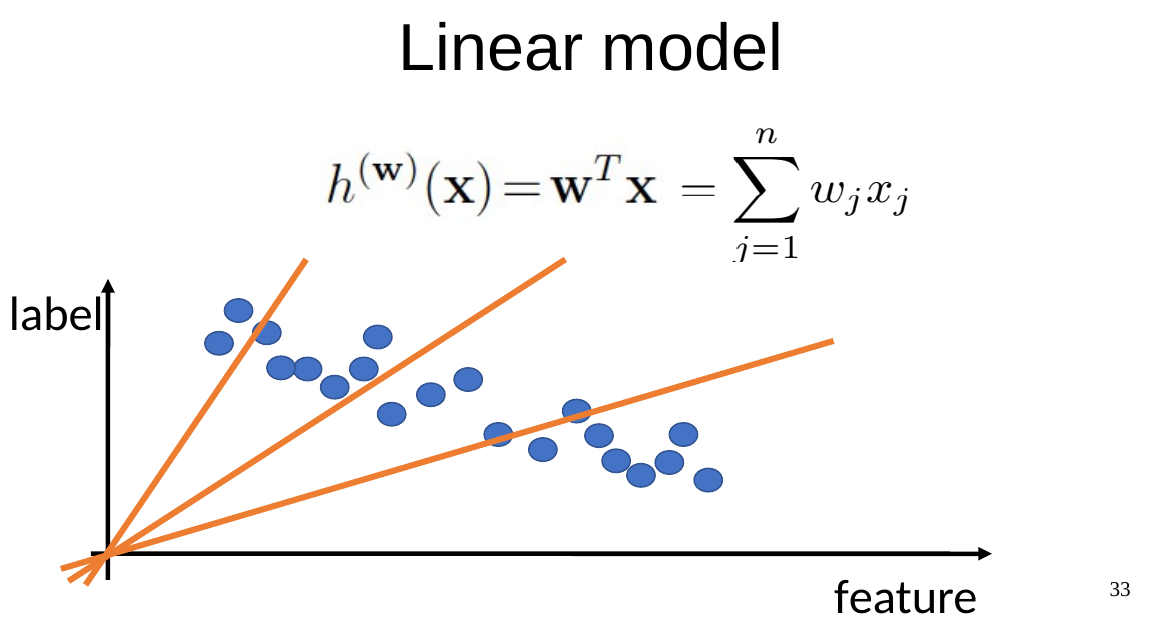
\includegraphics[width=1\linewidth]{images/3Comp/3comp2.png}
        \caption{}
        \label{fig:sub1}
    \end{subfigure}
    \begin{subfigure}{.4 \textwidth}
        \centering
        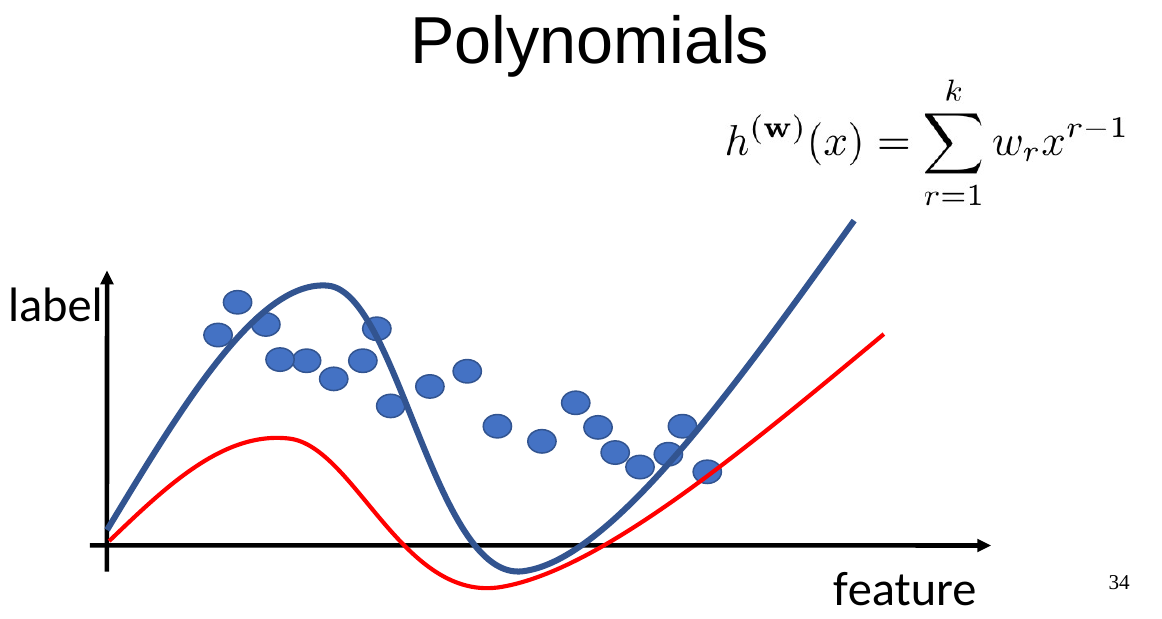
\includegraphics[width=1\linewidth]{images/3Comp/3comp3.png}
        \caption{}
        \label{fig:sub1}
    \end{subfigure}
    \caption{}
\end{figure}
\begin{figure}[H]
\centering
    \begin{subfigure}{.4\textwidth}
        \centering
        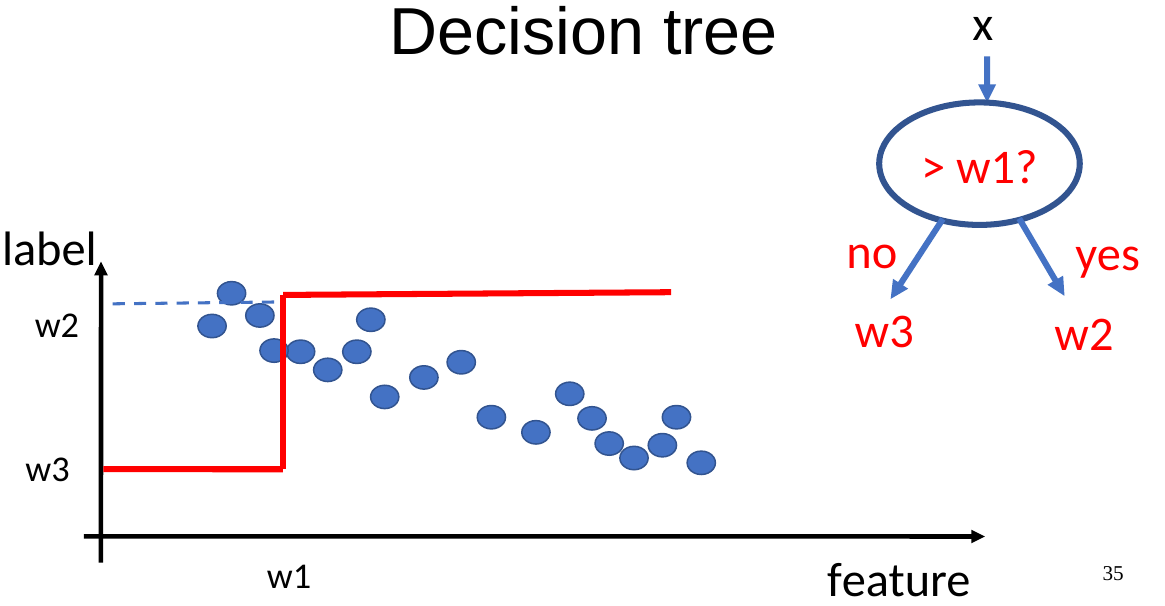
\includegraphics[width=1\linewidth]{images/3Comp/3comp4.png}
        \caption{}
        \label{fig:sub1}
    \end{subfigure}
    \begin{subfigure}{.4 \textwidth}
        \centering
        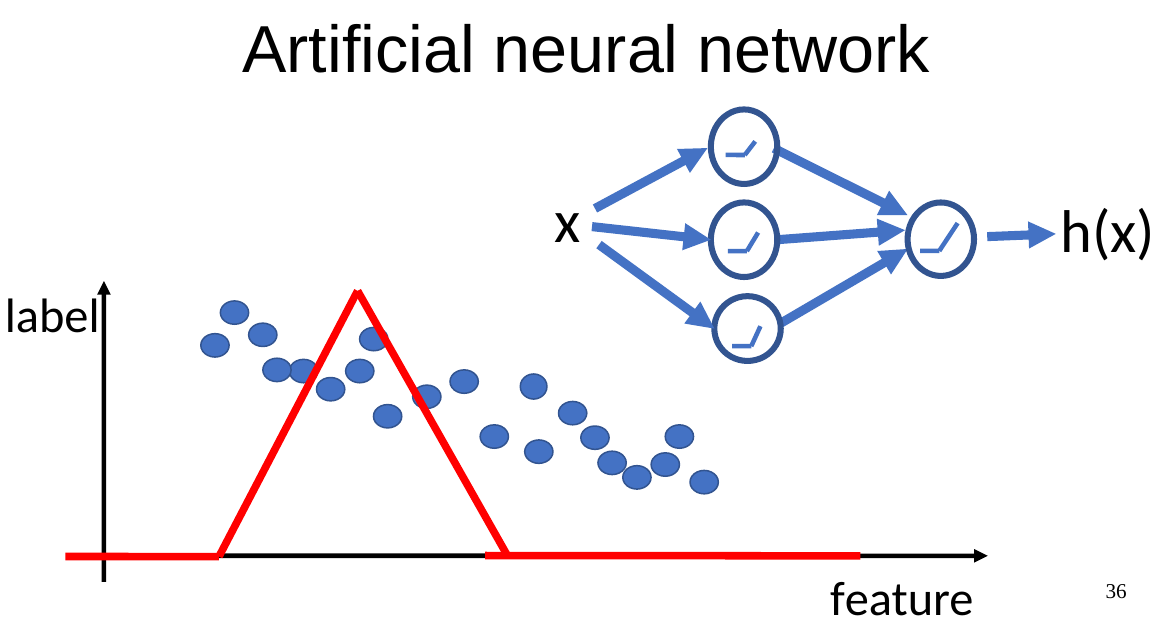
\includegraphics[width=1\linewidth]{images/3Comp/3comp5.png}
        \caption{}
        \label{fig:sub1}
    \end{subfigure}
    \caption{}
\end{figure}
To choose a model we have to consider and weigh 3 factors: \textbf{interpretability}, \textbf{computational} \textbf{complexity} and statistical accuracy, in fact the hypothesis has to be \textbf{sufficiently small} that means has much small as we can to have an optimal representation without overfit the model
\begin{figure}[H]
    \centering
    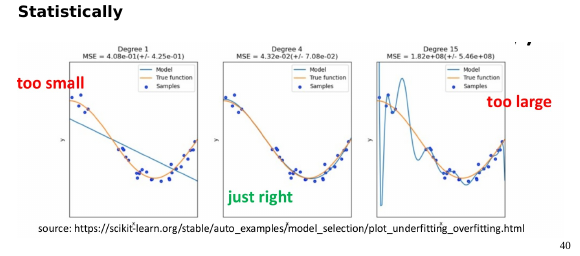
\includegraphics[scale=0.5]{images/3Comp/3comp6.png}
    \caption{Visual representation of sufficiently small}
    \label{fig:enter-label}
\end{figure}

\section{Loss}
The loss (funzione di costo in italiano) is the quantitative measure of prediction error obtained when using hypothesis h to predict label y’ of datapoint with features x’, there are different measure like the squared error loss $ L:= (\overline{y} - y)^2$ or the absolute error loss $L:= |\overline{y}-y|$. The binary classification is a different type which can have only a loss equal to 0 if we are correct and 1 if we did a mistake. As the model, choosing a loss function is done by considering: statistical aspects (should favour “reasonable” hypothesis), computational aspects (must be able to minimize them) and Interpretation (what does log-loss = -3 mean ?)

In conclusion to be able to learn from data and predict a label from new features we have to choose the right model with the right loss function
\begin{figure}[H]
\centering
    \begin{subfigure}{.4\textwidth}
        \centering
        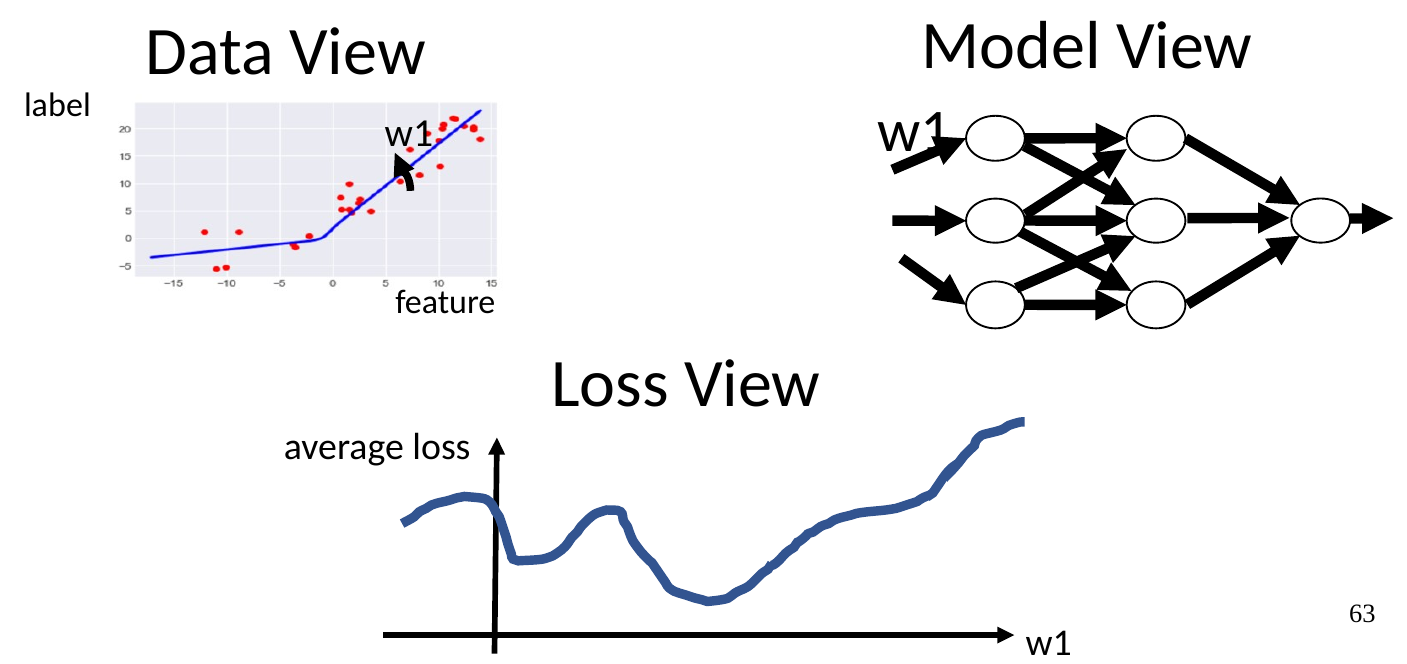
\includegraphics[width=1\linewidth]{images/3Comp/3comp7.png}
        \caption{Three views on machine learning}
        \label{fig:sub1}
    \end{subfigure}
    \begin{subfigure}{.4 \textwidth}
        \centering
        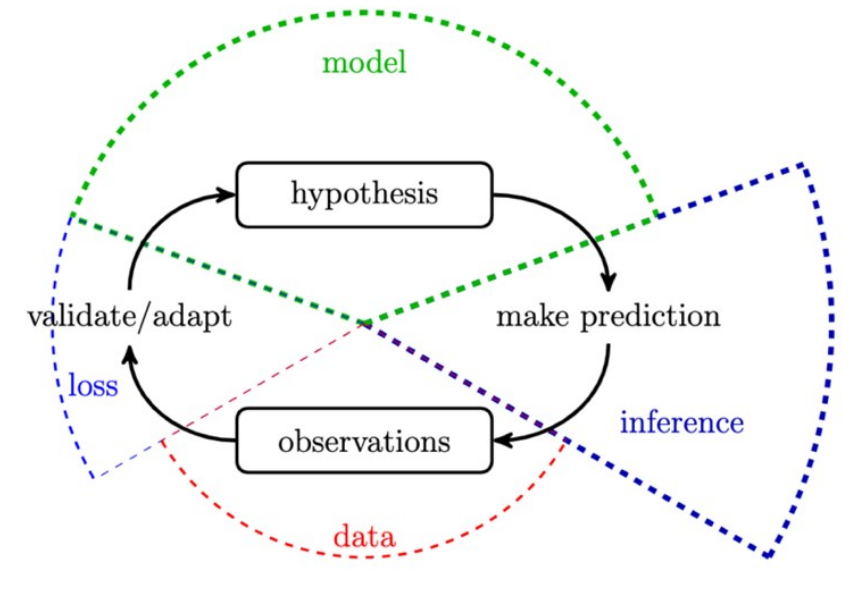
\includegraphics[width=1\linewidth]{images/3Comp/3comp8.png}
        \caption{ML process}
        \label{fig:sub1}
    \end{subfigure}
    \caption{}
\end{figure}


\chapter{Empirical Risk Minimisation}
We want an hypothesis$h \in H  h:X\rightarrow Y $ such that $h(x) \approx y$ for \textbf{any} data point $ (x,y)$, any datapoint means according to the distribution.
We want interpret the data point as realizations of i.i.d. random variables with probability distribution p(x,y) because the datapoint are part of the entire dataset. Define loss incurred for any data point as the expected loss, i.e., on average what will be the loss on the points of the distribution. Also called as \textbf{expected risk} or \textbf{Bayes risk}:
\begin{center}
    $E\{L((x,y),h)\} := \int_{x,y} L((x,y),h) d p (x,y) $
\end{center}
It is our integral weighted by the probability distribution. So to compute this expectation we need to know the probability distribution p(x,y) of data points (x,y).

However our goal is take the best hypothesis $h$ from the space of $H$ to minimize the expected loss, but estimate p(x,y) can be really difficult and not accurate, so the idea is approximate expected loss by average loss on data points (training set) called \textbf{empirical risk }.
\begin{center}
   Starting from Data $D = {(x^{(1)} , y^{(1)}), \dots , (x^{(m)} , y^{(m)})}$ with our m samples.\\
   We use that samples to compute the loss on the m samples $ \hat{L}(h|D) = \frac{1}{m} \sum\limits_{i=1}^m L((x^{(i)}, y^{(i)} ),h)$\\
   because for sufficiently larger (enough) sample size m $E\{L((x,y),h)\} \approx \Hat{L}(h|D) $\\
  \textbf{ \textit{learn hypothesis out of a hypothesis space or model that incurs minimum average loss when predicting labels of training datapoints based on their features}}
\end{center}
\begin{figure}[H]
    \centering
    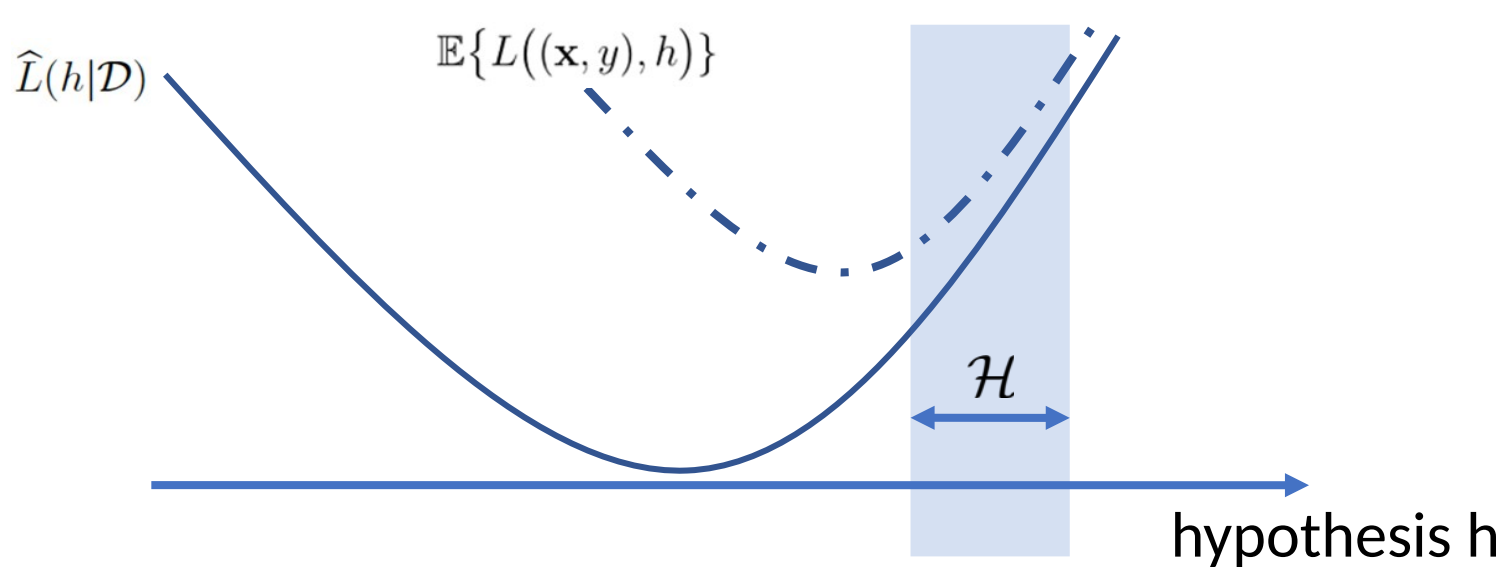
\includegraphics[scale=0.3]{images/ERM/ERM1.png}
    \caption{Empirical risk minimization}
    \label{fig:enter-label}
\end{figure}
In the picture above we have the 2 function of expected loss ($E$) and empirical loss ($L$) and our hypothesis $h$, but we have to consider only the $H$ space in light blue so the minimization of the 2 two function are equal in the left limit of $H$ that for both functions is closer to $h$.

If we have a parameterized function instead of considering the hypothesis space, so finding the best parameters instead of the best function we can transform $ h \in H \rightarrow w \in \mathbb{R}^n$.
\begin{center}
    With this change we can learnt parameters vector $\hat{w} = argmin f(w)$ with $ w\in \mathbb{R}^n$\\
  $  f(w) := \dfrac{1}{m} \sum\limits_{i=1}^m  L((x^{(i)}, y^{(i)} ),h^{(w)}) \rightarrow \hat{L} (h^{(w)} | \mathbb{D}) $ 
\end{center}
\begin{figure}[H]
    \centering
    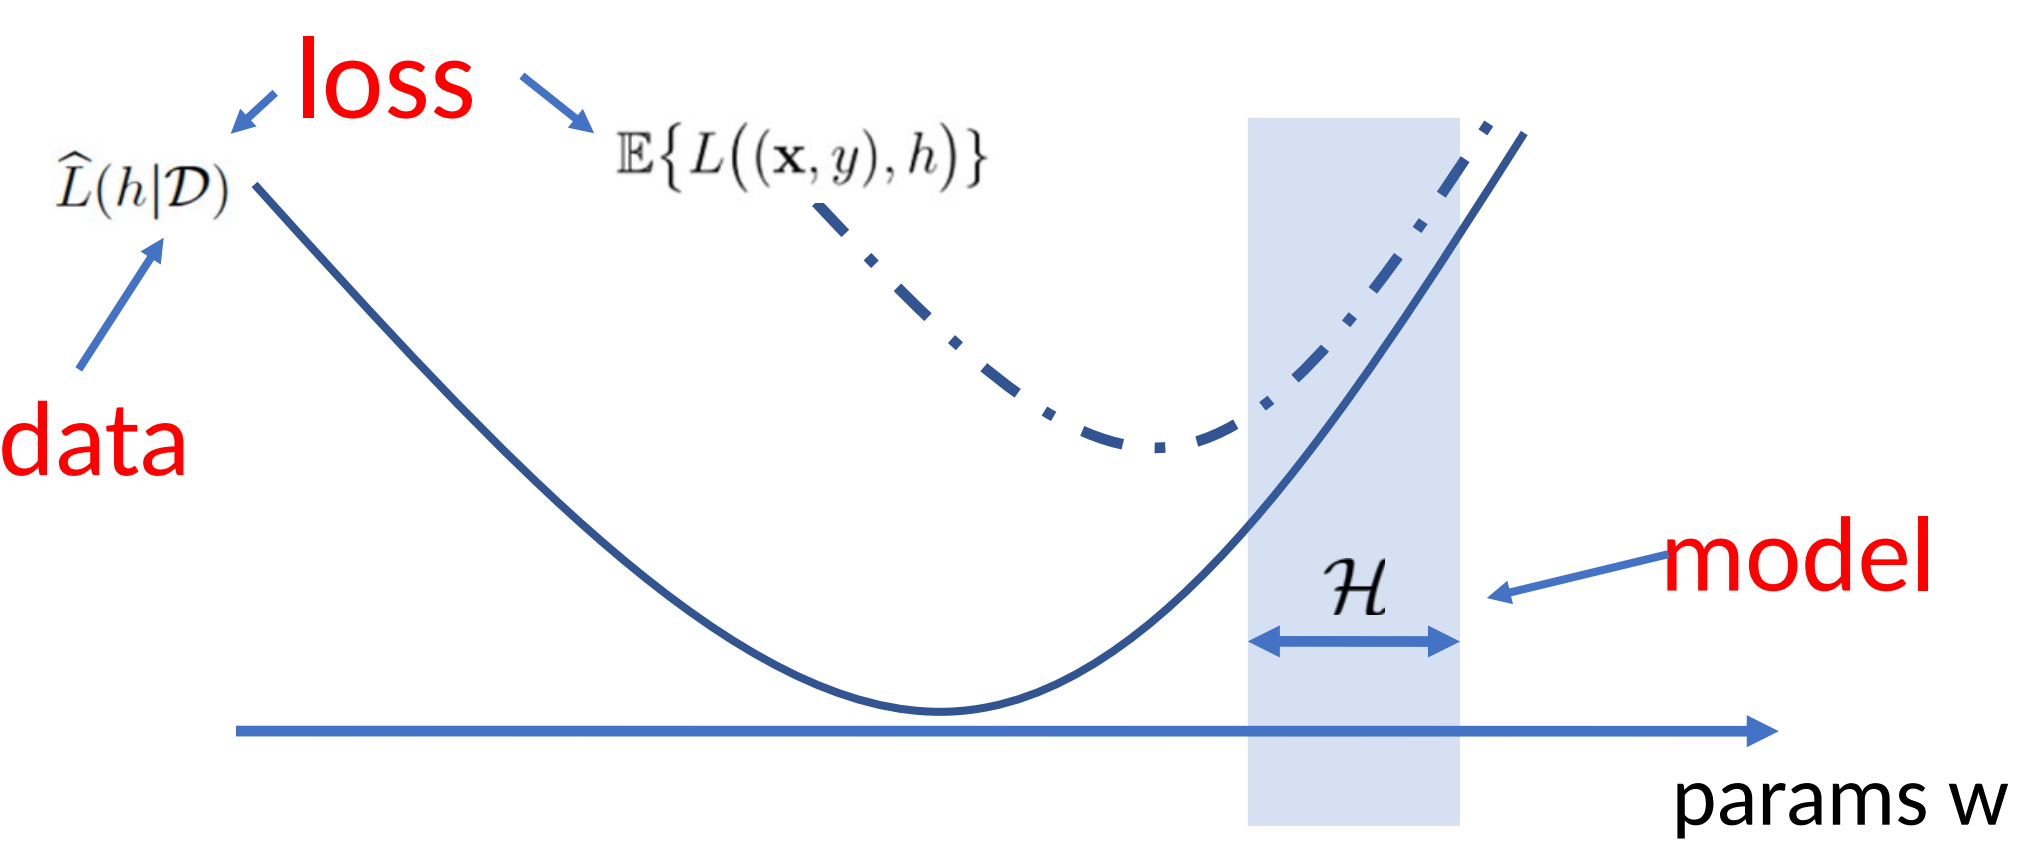
\includegraphics[scale=0.15]{images/ERM/ERM2.png}
    \caption{Design choices in erm}
    \label{fig:enter-label}
\end{figure}
 After all that assumption we can rewrite the machine learning definition :Learn a hypothesis in model that incurs in smallest empirical risk (loss) when predicting labels of training data points.
\section{Regression}
In any type of regression we have to define Data Model and loss, obviously in a regression the data can only have numeric type.

The formula has to work on the weights to apply on the n features that we have so the generic formula for the weights is: $ h^{(w)} (x) = w^T x= w_1 x_1+ \dots + w_n x_n$.\\
This is done to choose parameter/weight vector w to minimize average squared error loss or other error loss.\\
The example for linear regression became: $ \hat{w}= argmin (1/m) \sum\limits_{i=1}^i (j^{(i)} - w^T x^(i))^2 $
\begin{figure}[H]
    \centering
    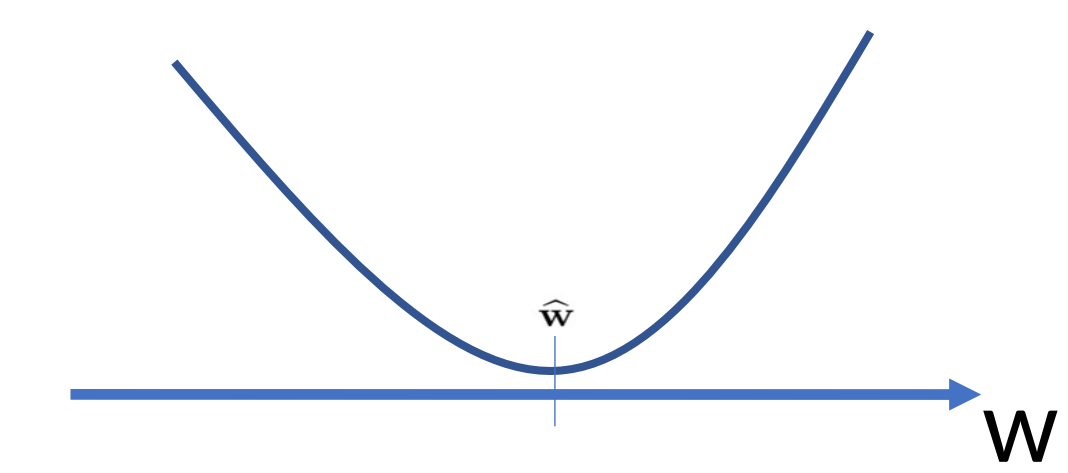
\includegraphics[scale=0.25]{images/ERM/ERm3.png}
    \caption{Example of linear regression with $\hat{w}$}
    \label{fig:enter-label}
\end{figure}

The feature map is a strategy that, starting from one single feature we create n feature applying different formulas to the single one, and than the process is the same to create a polynomial regression with different power up to the number of created features, creating bigger model with more flexibility:\\
$\mathbf{H}^{(n)}_{poly} = \{ h^{(w)}: \mathbb{R} \rightarrow \mathbb{R} : h^{(w)} (x) = \sum\limits_{j=1}^n x_j x^{j-1}$ with some $w = (w_1, \dots, x_n)^T \in \mathbb{R}^n  \} $
\begin{figure}[H]
    \centering
    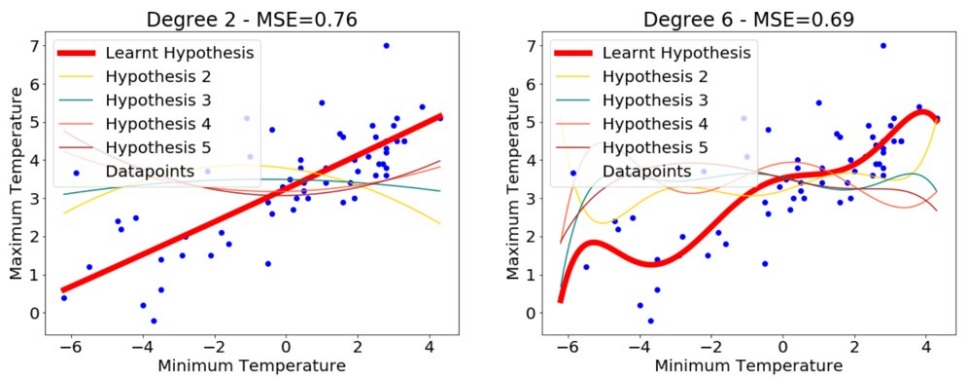
\includegraphics[scale=0.4]{images/ERM/ERM4.png}
    \caption{Comparison between degree}
    \label{fig:enter-label}
\end{figure}

There are different type pf calculating the error and we will see, as we already seen, the absolute, squared and a new one called Huber.

\begin{table}
    \centering
    \begin{tabular}{cccc}
         & Differentiable & Robust to outlier & Insensitive to noise \\
        Absolute loss & No & Yes & No\\
        Squared loss & Yes & No & Yes\\
        Huber loss & Yes & Yes & Yes\\
    \end{tabular}
    \caption{Caption}
    \label{tab:my_label}
\end{table}

All of them are convex function, but Huber loss merge them to use squared error loss when we are closer then $\epsilon$ and absolute error loss when we are further. Moreover this permit to don't depend on the outlier but have a more stable error function. The loss function have to be convex, because are simpler to minimize e differentiable for the same reason.
\begin{equation}
   L((x,y), h) =
    \begin{cases}
     (1/2)(y-h(x))^2 & for |y-h(x)| \ge \epsilon \\
     \epsilon (| y-h(x)| - \epsilon/2)\ & else
    \end{cases}       
\end{equation}

\section{Classification}

In classification we don't have number so we can't use the distance or function in same space, we have to obtain them through confidence measures. The output will be a label or multi-label.

Data points with numeric features, same as in linear regression. Model = space of linear maps, same as in linear regression; the change is in Logistic loss that is different from linear regression.

We need a formula that changes according to the output as $ L((x,y) ,h) := log (1+exp (-yh(x))) $, with squared error loss we can't because we aren't change between the two part (less and more than 0 ) of the function.

\begin{figure}[H]
    \centering
    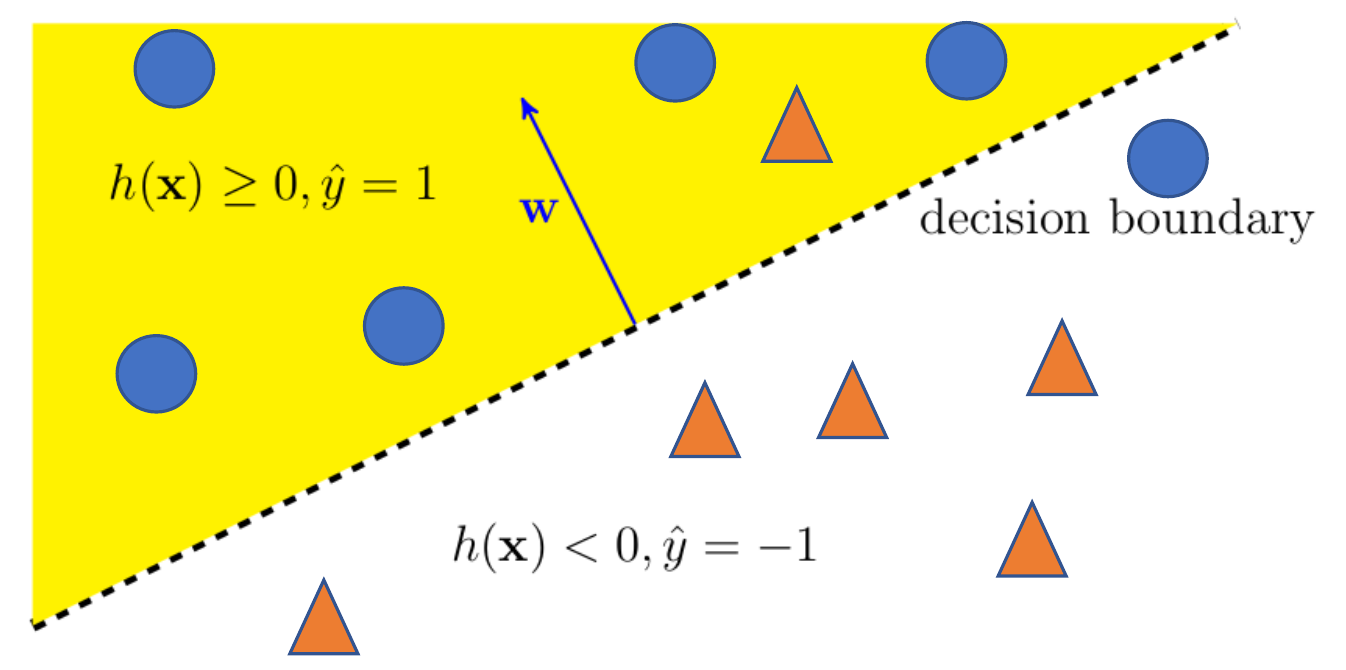
\includegraphics[scale=0.3]{images/ERM/ERM5.png}
    \caption{Logistic regression}
    \label{fig:enter-label}
\end{figure}


\paragraph{Losses in classification:}: the 0/1 loss isn't differentiable and non convex, 
\begin{equation}
   L((x,y), h) =
    \begin{cases}
     1 & for y \ne \hat{y} \\
     0 & else
    \end{cases}       
\end{equation}

Hinge loss $L((x,y), h) := max \{ 0,1 - yh(x) \}$, it is convex but non differentiable

\begin{figure}[H]
    \centering
    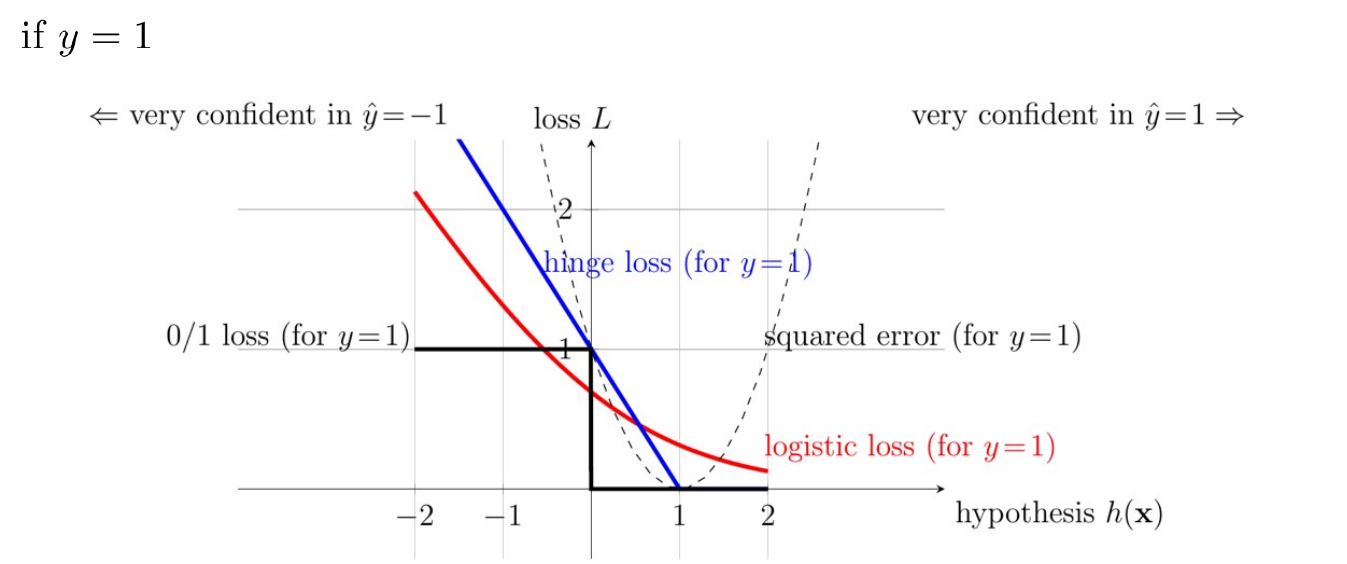
\includegraphics[scale=0.4]{images/ERM/ERM6.png}
    \caption{Comparison between losses}
    \label{fig:enter-label}
\end{figure}
\chapter{Model Validation and Selection}

Choosing different exponential for the Hypothesis $H^0$ or $H^3$ we are changing the different shape of our function and every bigger polynomial contain the smaller one.
The question is, it is better to work with a smaller exponent or a bigger one? We can measure that with the sum of the error of all the point that we have, and in that case we can say that bigger polynomial can lower the \textbf{training} error made in the training set. In general at some degree our error can became equal to 0, but in that case we made an error called \textbf{overfitting}.
We can't specialized so much on our training data because the other data aren't as the training so small train error \textbf{does not guarantee good performance} outside the training set.
It is important to create another subset of data called \textbf{validation set}, the purpose of this subset is to probe the hypothesis we did in the training set with other data to see the performance.
The real importance is to divide the data we use to take the hypothesis and the  one to probe that the hypothesis work.

\begin{figure}[H]
    \centering
    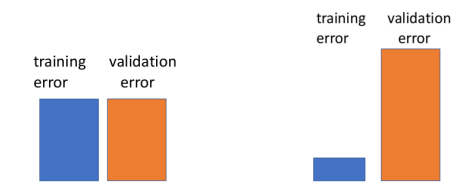
\includegraphics[scale=0.4]{images/MVS/MVS1.png}
    \caption{Example of validation error}
    \label{fig:enter-label}
\end{figure}

The aim is to reach the perfect balance without underfitting or overfitting so the lowest point on the training error and validation error to reach the correct number of complexity.
\begin{figure}[H]
    \centering
    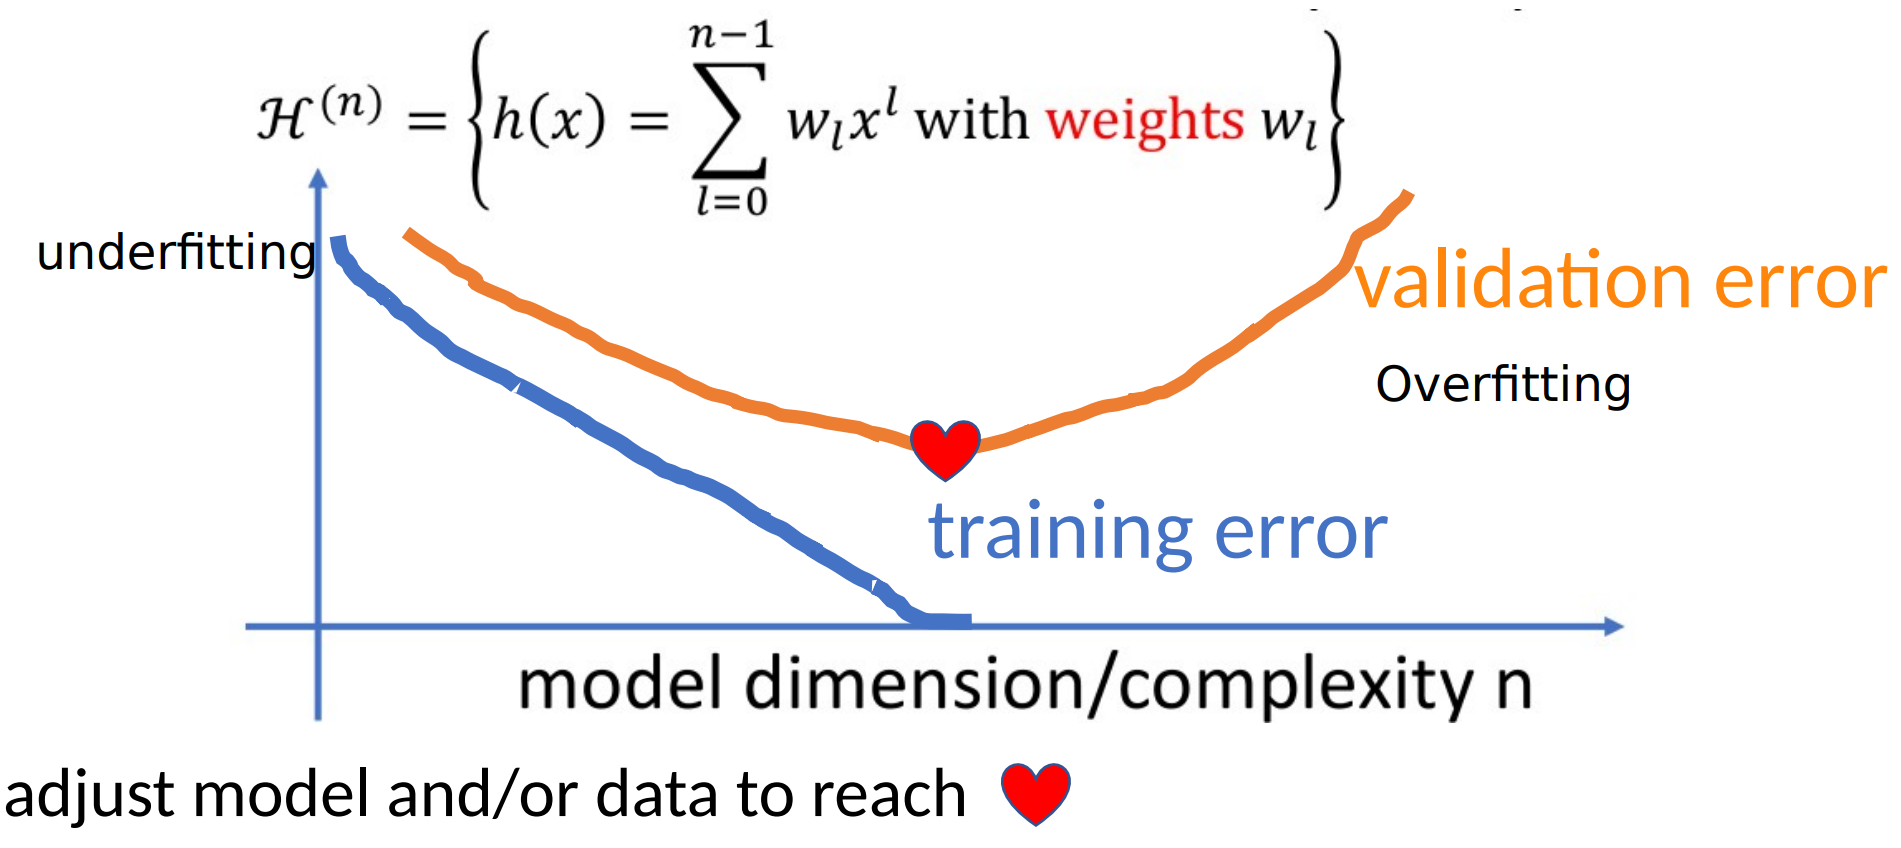
\includegraphics[scale=0.25]{images/MVS/MVS2.png}
    \caption{Train/Val Error vs. Model Complexity}
    \label{fig:enter-label}
\end{figure}

Another type of possible validation is the k-fold cross validation, the idea is to randomly split several times the data in different ways. The training error is the average empirical loss over the k training folds and the validation error is the average empirical loss over the k validation folds. Obviously the key is choose the number of folds because the train fold should be sufficiently large and the validation folds should be sufficiently large. there are also different type of k-fold like class-ratio preserving splitting, group-preserving splitting or temporal successive splitting

\begin{figure}[H]
    \centering
    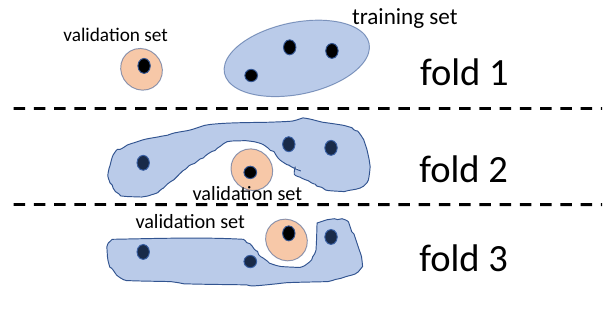
\includegraphics[scale=0.4]{images/MVS/MVS3.png}
    \caption{k-fold cross validation}
    \label{fig:enter-label}
\end{figure}

The test set is chosen model with validation error, Need a test set different from training and validation set.

The action to do are: 
\begin{itemize}
    \item input: list of candidate models
    \item  for each candidate model
        \begin{itemize}
            \item learn optimal hypothesis by minimize training error
            \item compute validation error on validation set
        \end{itemize}
    \item choose hypothesis with minimum validation error
    \item  compute test error of on test set
\end{itemize}
\chapter{Metrics hyperparameter tuning}

After taking the best possible loss minimizing ERM and tuning the parameters we want to have something humans readable so we use metrics that are measure of quality of our choice.
The evaluation of supervised Machine learning are different:
\begin{enumerate}
    \item efficiency
    \item scalability
    \item robustness
    \item interpretability
\end{enumerate}

The quality of the prediction is different from the prediction one, there are:
\begin{enumerate}
    \item Confusion matrix
    \item Accuracy 
    \item Precision 
    \item ROC curve
\end{enumerate}
\subsection{Confusion matrix}
\begin{figure}[H]
    \centering
    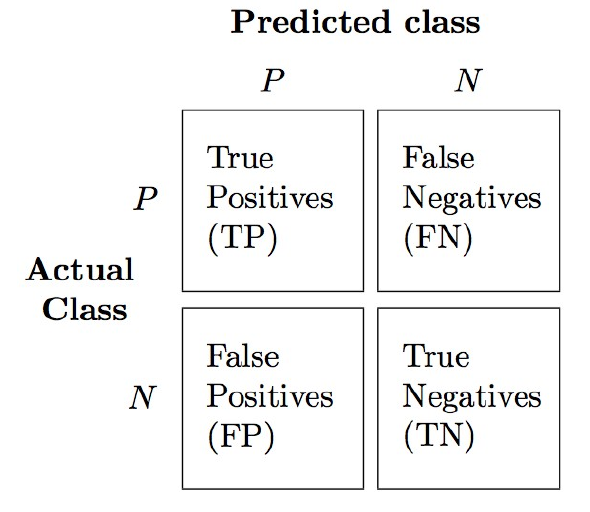
\includegraphics[scale=0.3]{images/PM/PM1.png}
    \caption{Example of confusion matrix for binary classifier}
    \label{fig:enter-label}
\end{figure}

\subsection{Accuracy}
It is the most widely-used metric for model evaluation: $acc = \dfrac{\text{Number of correctly classified obj}}{\text{Number of classified obj}}$ and for binary classifiers became : 
$ Accuracy = \dfrac{\text{TP + TN}}{\text{TP + TN + FP + FN}}$. The one related to 0/1 loss is: $ 1- (1/m) \sum\limits_{i=1}^m L((x^{(i)}, y^{(i)}),h) $.

Accuracy might be misleading when we have not balanced samples and maybe a missclassification for some objects of a given class could have different importance like in medical problem. For this problem we can use other correlated measure like \textbf{precision}:
$ p = \dfrac{\text{Number of objects correctly assigned to c}}{\text{Number of objects assigned to c}}$ or $ p = \dfrac{TP}{TP+FP}$ 

and the \textbf{recall}:
$ \dfrac{\text{Number of objects correctly assigned to c}}{\text{Number of objects belonging to c}}$ or $ r = \dfrac{TP}{TP+FN}$. Precision measure how many selected items are relevant and the recall measure how many relevant items are selected; both are measure applied to \textbf{every class}. Combining them we can have F-measure: $F = \dfrac{2rp}{r+p} $ or $F=\dfrac{2TP}{2TP + FP +FN}$ that is the harmonic mean.

\subsection{ROC curve}
ROC (Receiver Operating Characteristics) developed for noisy signals to find the trade-off between positive hits and false alarms.

\begin{figure}[H]
    \centering
    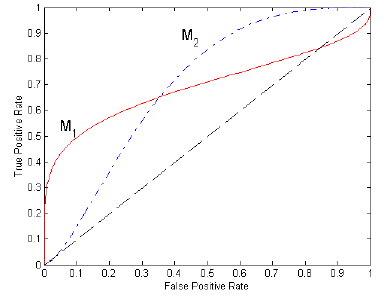
\includegraphics[scale=0.6]{images/PM/PM2.png}
    \caption{ROC curve, each point is a different Hypothesis. Ideally we want to stay in the top left corner but we can't so we have to choose the trade-off as humans}
    \label{fig:enter-label}
\end{figure}

Normally we choose the one with more area under the function (integral) if we don't have constraint. This is called AUC ROC curve.


\section{Learning curve}
\chapter{Gradient learning}

Small math reminder $\nabla$ indicates derivatives: the derivatives on a function indicates the gradient (pendenza) on a point in the function so if positive we are growing in that point, if negative we are falling. Since we are using parable we only have 1 point with the derivatives = 0. 
\section{Gradient based learning}
Now we want to find the ERM on parametrized models, basically we want the minimum of the parametrized function. To achieve that we will use the gradient based method which consist in a iterative method that change based on what we obtain in the previous iteration.
What we have to do is construct a sequence of parameter vectors $w(0) \rightarrow w(1)$ that hopefully converge to a minimizer of f(w): $ f(\overline{w}) = \overline{f} := min f(w) $.

We approximate  locally $f(w)$ around $w^{(r)}$: $ f(w)\approx f(w^{(r)}) + (w-w^{(r)})^T \nabla f (w^{(r)})$ for w sufficiently close to $ w^{(r)}$.\\
Since we want to minimize f, we should go in the direction w such that $(w-w^{(r)})^T \nabla f (w^{(r)})$ is negative.\\
The next step has to be, given current guess w(r): $w^{(r +1)} = w^{(r)} - \alpha \nabla f(w^{(r)}) $ with a sufficiently small step size $\alpha >0$ and with $\alpha$ called learning rate.
\begin{figure}[H]
    \centering
    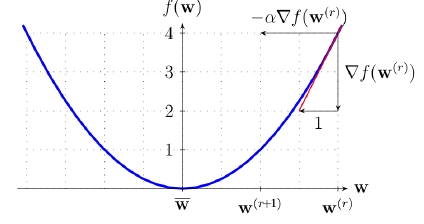
\includegraphics[scale=0.7]{images/GB/GB1.png}
    \caption{If $\nabla f(w^{(r)}) $ is positive, so in the right part of the minimum we have to go back in the left side with $- \alpha \nabla f(w^{(r)})$ called correction term, it will be the same if $\nabla f(w^{(r)}) $ was negative}
    \label{fig:enter-label}
\end{figure}

\subsection{Example: GD for linear regression}

We already know the ERM for linear regression that is $ \overline{w} = argmin f(w)$ with $  f(w) := \dfrac{1}{m} \sum\limits_{i=1}^m ( y^{(i)} - w^T x^{(i)})^2 $\\
If we compute gradient we obtain: $ \nabla f(w) = - \dfrac{2}{m} \sum\limits_{i=1}^m ( y^{(i)} - w^T x^{(i)}) x^{(i)} $\\
Then the gradient step is $ w^{(r)} := w^{(r-1)} + \alpha \dfrac{2}{m} \sum\limits_{i=1}^m ( y^{(i)} - w^T x^{(i)}) x^{(i)}$
\subsection{Choosing learning rate}
The problem now is,  how much is $\alpha$ need to be? It depends on the implementation and where we are because sometimes could be useful have big $\alpha$ to have a large step size and sometimes small step are recommended. In some cases, theoretical bounds and optimal values can be given but is \textbf{proved} that number of GD steps is smaller for standardized data. Another problem is when to stop, the solution can be have a fixed number of iteration (epochs) or when $ f(w^{(r-1)} ) - f(w^{(r)}) $ is less than a threshold or when validation error keep decreasing.

\section{Stochastic gradient descent}

The idea is to not use all the samples that could be billions, but use an approximation of the gradients descend :
\begin{itemize}
    \item Iteratively replace sum with a (random) component \\
    $g(w) := \nabla f_{i}(w) \quad w^{(r+1)} = w^{(r)} - \alpha \nabla f_{ir} (w^{(r)})$ 
    \item Iteratively replace sum with a (random) batch\\
    $ \mathbb{B} = \{ i_1, \dots , i_b\}  $ as batch $\quad g(w) = \dfrac{1}{\mathbb{B}} \sum\limits_{i' \in \mathbb{B}} \nabla f_{i'} (w)$
\end{itemize}

The idea is, instead of have less step on large samples is can be better have more step on fewer samples.

\section{Multi class classification}

Not all the classification can be binary but we want to have more label possible, often at the same time. There are different approach:
\begin{itemize}
    \item Naive approach: consider each label separately and solve problem separately for each label ignoring correlation (One vs rest trick)
    \item Multi class approach where each combination of label define a different categories, this means that the number of categories will be bigger
    \item Multi task learning approach: each individual label results in separate learning task and then combine the loss to learn together the two hypothesis
\end{itemize}

\section{Supervised learning techniques}
The supervised learning techniques can be divided into 2 different classes: the \textbf{regression} and the \textbf{classification}

\subsection{Regression}
\subsubsection{LASSO regressor}
LASSO (Least absolute shrinkage and selection operator) use regressor on a space of linear maps with datapoints with numerical features and label, the loss is the regularized squared loss.
Linear regression requires a training set larger than the number of features (m>n) to not overfit, but this is not a big issue considered that we can use regularization techniques with  penalty term in the loss for using too many features.\\
$L((x,y),h^{(w)} ) = (y -w^Tx)^2 + \lambda ||w||_{1} \rightarrow $ Increasing $\lambda$ results in a weight vector w with increasing number of zero coefficients and Works as a feature selection


\subsection{Classification}
\subsubsection{Support Vector Machines}

It is a classifier that can be extended as regressor and the datapoint must be numeric feature. The label values have to be binary; the model is a space of linear maps and the loss is the regularized hinge loss. The idea is to maximize the margin between different object in the hyperplane. The margin is the minimum distance of all closest point (missclassified have negative distance)
\begin{figure}[H]
    \centering
    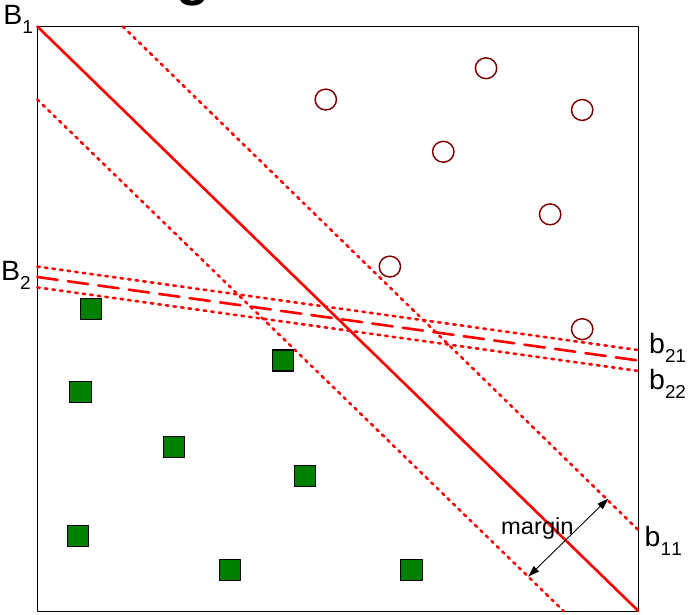
\includegraphics[scale=0.3]{images/GB/GB3.png}
    \caption{Caption}
    \label{fig:enter-label}
\end{figure}

The loss favors linear maps h(w) that are robust against (small) perturbations of the data points – more robust than logistic regressor

\subsubsection{Naive Bayes classifier}

Bayes classifiers are classifier that from a datapoint with numeric features give a 0/1 loss for every label using the Bayes rules ($ p(y|x) = \dfrac{p(x|y)* p(y)}{p(x)}$), the only problem is that We do not have this probability distribution $\rightarrow$ estimate it from training points because p(x) is constant for all y; p(y) is estimated by relative frequency of class y in the training set, but for p(x|y) we can only estimate

\begin{figure}[H]
    \centering
    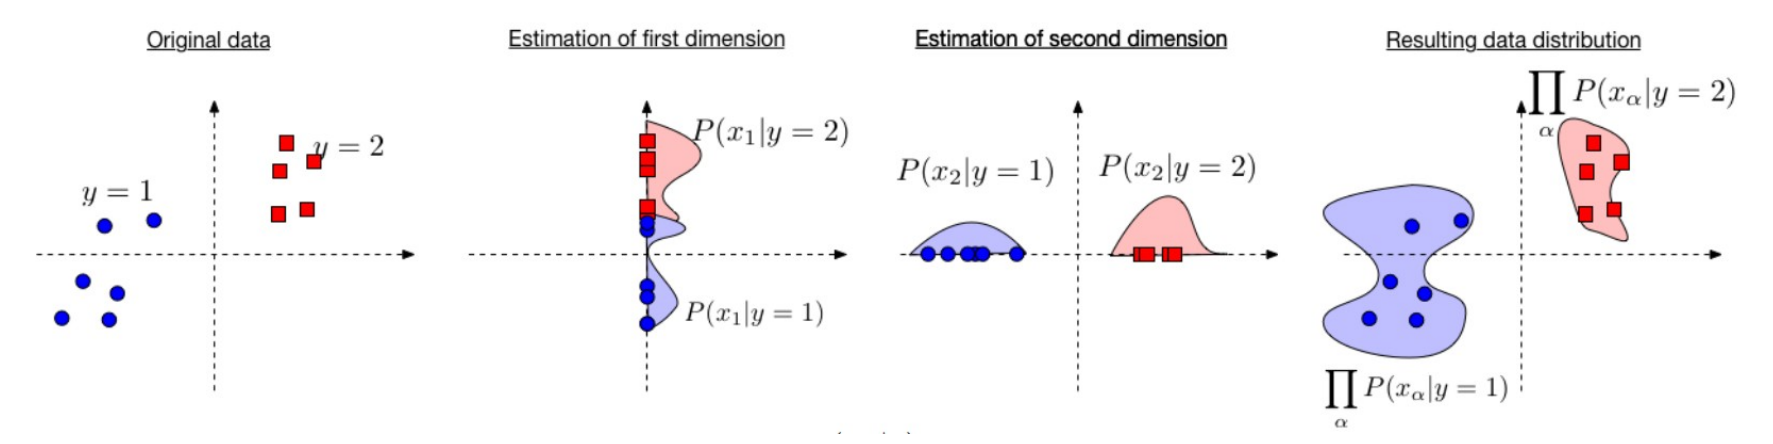
\includegraphics[scale=0.3]{images/GB/GB4.png}
    \caption{Caption}
    \label{fig:enter-label}
\end{figure}

$ h(x) = argmax_y p(y|x) = argmax_y \dfrac{p(x|y)* p(y)}{p(x)} $\\
$= argmax_y p(x|y)* p(y)$ because p(x) doesn't depend on y \\
$= argmax_y \prod\limits_{\alpha=1}^d p(x_{\alpha}|y)* p(y)$ by the naive Bayes assumption\\
$= argmax_y \sum\limits_{\alpha=1}^d log(p(x_{\alpha}|y)) * log(p(y))$ as log is a monotonic function

It is important to know that Naive Bayes is a linear classifier and a variant called Gaussian Naive Bayes where we assume x as a Gaussian with mean and variance depending on y
\subsubsection{Decision Tree and Random Forest}
Decision tree are models that uses a tree-like model of decisions and their possible outcomes/classes and contains only conditional control statements. There are many algorithms like Hunt's, CART, ID3 C4.0, C5.0. Are useful because allows non-linear regression and are very fast and easy to interpret.  In regression, the trees output a single number per leaf node instead of a label.

Random forest  is an ensemble classifier that consists of many decision trees, For each tree of the K trees of the forest, choose a subset of n’ features (n is the total number of features) and a subset of m’ training data (m is the total number of samples)
 \begin{figure}[H]
     \centering
     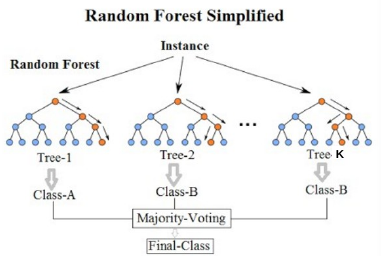
\includegraphics[scale=0.8]{images/GB/GB6.png}
     \caption{Caption}
     \label{fig:enter-label}
 \end{figure}
 There is also a visualizer for them.
\subsubsection{K-nearest neighbors}
 Uses k closest points for performing classification/regression, the choice of the k is important because too big or too small can cause problem.
 \begin{figure}[H]
     \centering
     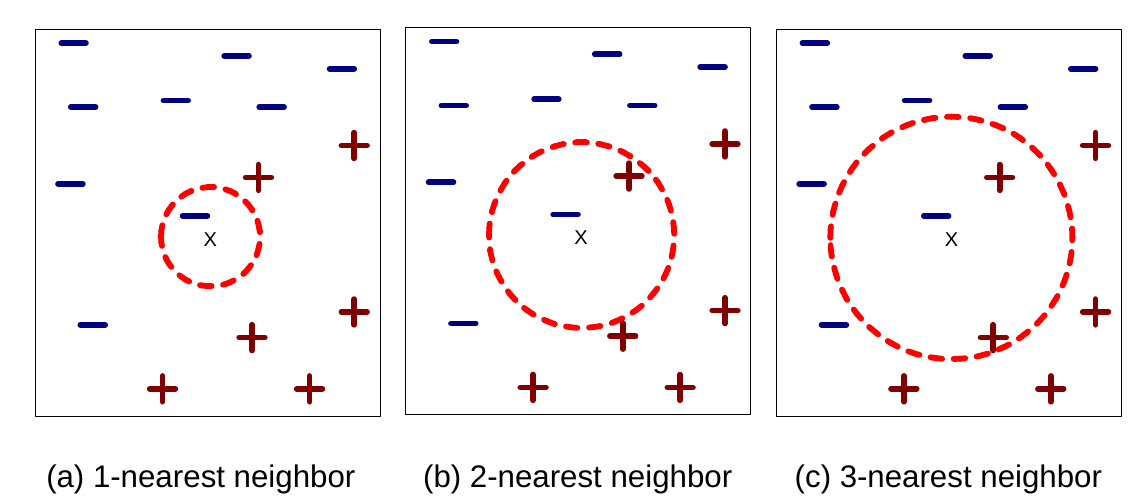
\includegraphics[scale=0.5]{images/GB/GB5.png}
     \caption{Caption}
     \label{fig:enter-label}
 \end{figure}
\chapter{Unsupervised learning: Cluster}
That type of learning is called unsupervised because we have No labelled data points, No ground truth to compare with. A cluster corresponds to a subset of data points that are in some sense homogeneous or similar. The definition of a cluster is ambiguous because anyone can see different cluster over the same image of amount of data, so we have the difference between \textbf{hard clustering} and \textbf{soft clustering}
\section{Hard clustering}

Hard clustering methods compute predicted cluster indices $\hat{y}^{(i)}$ based solely on features $x^{(i)}$, in theory there is a true label but we can't use it.
Our algorithm has to take only the feature vectors to predict the cluster assignments

In some clustering method called k-means clustering algorithm there is the parameter k that indicates the number of cluster we want before the computation. Each cluster is associated with a \textbf{point} (mean or centroid)
\begin{figure}[H]
    \centering
    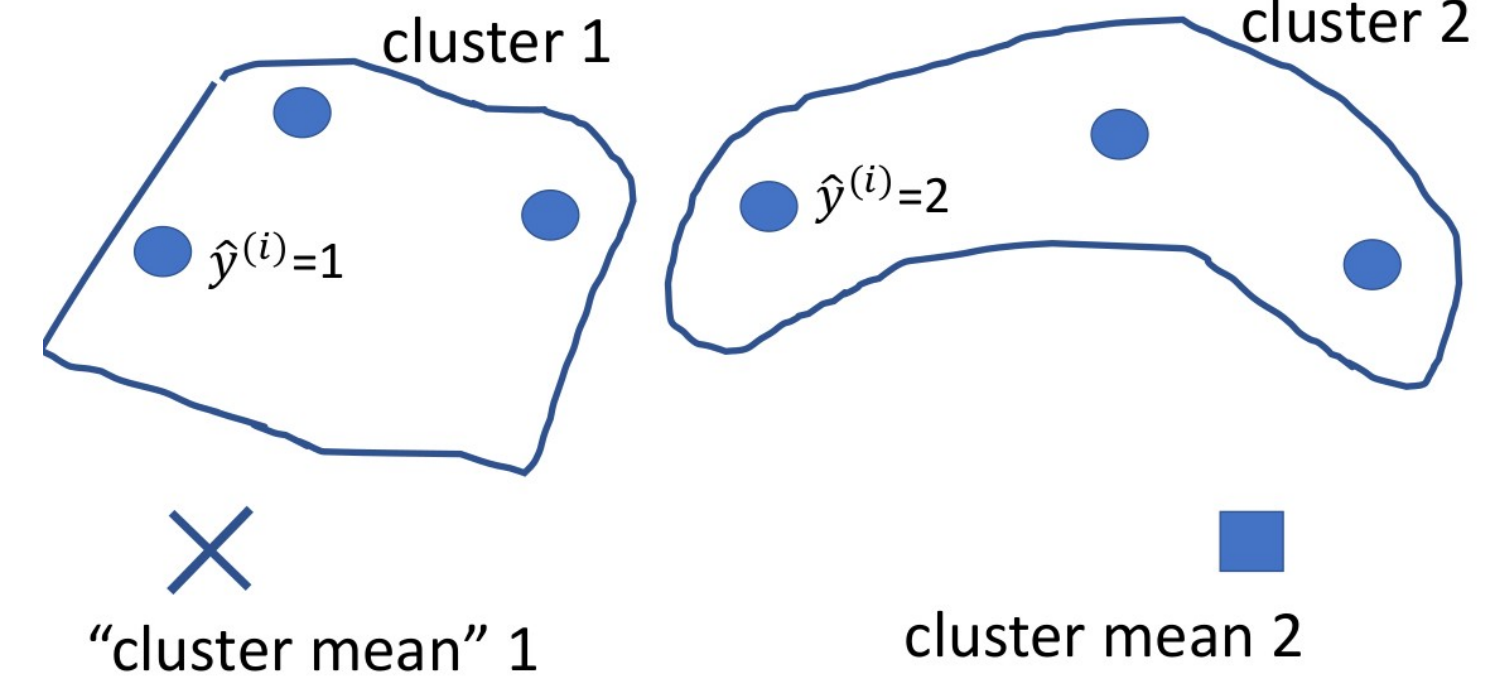
\includegraphics[scale=0.3]{images/CL/CL1.png}
    \caption{Caption}
    \label{fig:enter-label}
\end{figure}

We can measure the cluster spread through Average squared Euclidean distance between points and mean of cluster $ C^{(i)}$ :\\
Spread for a cluster: $ \dfrac{1}{|C^{(i)}|}  \sum\limits_{i\in C^{(i)}}^m || m^{(i)} - x^{(i)}||^2$ \\
Error in general with all the k cluster: $ \dfrac{1}{m} \sum\limits_{c=1}^k \sum\limits_{i \in C^{(C)}} || m^{(c)} - x^{(i)}||^2$

For given cluster means, clustering error is minimized by assigning $i^{th}$ data point to cluster with \textbf{nearest cluster mean} and for given cluster assignments, clustering error is minimized by representing $c^{th}$ cluster by the cluster mean of feature vectors of its data points

\begin{figure}[H]
    \centering
    \includegraphics[scale=0.5]{images/CL/CL2.png}
    \caption{Caption}
    \label{fig:enter-label}
\end{figure}

The clustering error, to be minimized is an empirical risk minimization problem.\\
$ \epsilon ( \{ m^c \} , \{ \hat{y}^i \}) := \frac{1}{m} \sum\limits_{i=1}^m || m^{(\hat{y}^(i))} - x^{(i)}||^2  $\\
Simultaneously finding cluster means m(c) and assignments that minimize clustering error is difficult to complete, in fact it is NP-hard.
The solution is not solve the 2 problem together:
\begin{itemize}
    \item For given assignments, finding cluster means that minimize clustering error is easy
    \item  For given cluster means, finding assignments that minimize clustering error is easy
\end{itemize}

The cycle function will be like this:
\begin{enumerate}
    \item Input: number k of clusters, initial cluster means
    \item update cluster assignments
    \item update cluster means
    \item Go to step 2 until finished
    \item Output: final cluster means
\end{enumerate}

An important rules is that we can't increase error in our cycles, the error can only decrease or be the same. But the initialization is very important because a bad initialization can converge into a local optimum but not the optimal clustering because we can have multiple minimum.

\begin{figure}[H]
    \centering
    \includegraphics[scale=0.3]{images/CL/CL3.png}
    \caption{In the first image we have a good initialization in the second no}
    \label{fig:enter-label}
\end{figure}

To avoid that problem we can run some iteration with different initialization and choose the best; another problem could be choosing the k number of clusters and it could be done with the elbow method or given from the type of problem we have. Another method is to choose k by validation error with different value of k


\section{Soft clustering}
Indeed in soft clustering every datapoint is characterized by k label values, multilabel. Every value is a degree of the point belonging to cluster 1 to k. The value are between 0 and 1 and the results are a probability of being in a cluster or not.

\subsection{Gaussian mixture model}
 Each cluster produces data based upon random draws from a (multi-dimensional) Gaussian distribution and  should be less likely to have data at the edge, each Gaussian cluster has its own mean and standard deviation
\begin{figure}[H]
\centering
    \begin{subfigure}{.4\textwidth}
        \centering
        \includegraphics[width=1\linewidth]{images/CL/CL4.png}
        \caption{}
        \label{fig:sub1}
    \end{subfigure}
    \begin{subfigure}{.4 \textwidth}
        \centering
        \includegraphics[width=1\linewidth]{images/CL/CL5.png}
        \caption{}
        \label{fig:sub1}
    \end{subfigure}
    \caption{}
\end{figure}
Mean vector: $ \mu$, covariance matrix $\Sigma$ \\
Gaussian distribution: $ \dfrac{e^{-\frac{1}{2} (x-\mu)^T \Sigma^{-1} (x-\mu )}}{\sqrt{(2\pi)^n det(\Sigma)}}$\\
Cluster spread: $\frac{1}{m^{(c)}} \sum\limits_{i=1}^m \hat{y}_c^i (x^i - \mu^c )^T  (\Sigma^1)^{-1} (x^i - \mu ^c) $\\
Means :$ \mu^c := \frac{1}{m^{(c)}} \sum\limits_{i=1}^m \hat{y}_c^i x^i $ for all c=1..k\\
Covariance: $\Sigma^C := \frac{1}{m^{(c)}}  \sum\limits_{i=1}^m  \hat{y}_c^i (x^i - \mu^c )^T (x^i - \mu ^c)$\\
Cluster assignment update: $  \hat{y}_c^i := \dfrac{m^c p(x^i| \mu^c , \Sigma^c )}{\sum\limits_{c'=1}^k m'^c p(x^i| \mu'^c , \Sigma'^c)} $


The algorithm is similar to the hard clustering updating in different moment in a loop until we resolve that.

\begin{itemize}
    \item INPUT: $(x^1, \dots , x^m), k, \{ \mu^c, \Sigma^c, m^c \} $
    \begin{enumerate}
        \item  Update soft cluster assignments $\hat{y}_c^i$
        \item Update cluster params $ \mu^c, \Sigma^c, m^c $
        \item Go to 1. unless “finished”
    \end{enumerate}
    \item OUTPUT: $\hat{y}_c^i, \mu^c, \Sigma^c, m^c $
\end{itemize}

The error: $ \epsilon := \sum\limits_{i=1}^m log \sum\limits_{c=1}^k  \frac{m^c}{m} p(x^i| \mu'^c , \Sigma'^c) $ This is negative logarithm of probability to sample data points under Gaussian mixture mode and it is equal to maximize likelihood; this is an Empirical Risk Minimization problem.

As in k-means we have the same problem about the initialization and the stop for cycle.
\subsection{Connectivity based clustering}
 k-Means and GMM fails on non-Euclidean cluster structure and cannot recognize outliers/noise. So we can use other types of clustering based on graph.  Connect close-by data points obtaining an empirical graph.
 This method use hard clustering and are 2:
 \begin{itemize}
     \item Spectral clustering: Eigenvectors of graph Laplacian matrix to measure connectivity between nodes
     \item DBSCAN: Density based spatial clustering with noise
 \end{itemize}

 \subsubsection{DBSCAN}
Data points need to be connected via core points, Core points are the ones with a minimum number of neighbors, Automatically determines number of k clusters. The outlier will be automatically discarded
It will accept 2 parameters:
\begin{itemize}
    \item Epsilon: Maximum distance to be connected
    \item MinPts: Minimum number of points to be a core point
\end{itemize}

\begin{figure}[H]
    \centering
    \includegraphics{images/CL/CL6.png}
    \caption{Caption}
    \label{fig:enter-label}
\end{figure}

\subsubsection{Hierarchical clustering}
A set of nested clusters organized as a hierarchical tree (dendogram); Any desired number of clusters can be obtained by ‘cutting’ the dendogram at the proper level and Different levels may correspond to meaningful taxonomies Key operation is the computation of the proximity of two clusters
\begin{figure}[H]
    \centering
    \includegraphics{images/CL/CL7.png}
    \caption{Caption}
    \label{fig:enter-label}
\end{figure}

\subsection{Comparing clustering}

We can measure a cluster validity using different index:
\begin{itemize}
    \item Internal Index: goodness of a clustering structure without external information (Ex: Silhouette index, sum of squared error (k-Means), log-likelihood)
    \item External or Relative Index: extent to which cluster labels match externally supplied class labels or labels from another clustering (Ex: entropy, purity, rand-index, adjusted rand-index, mutual information, adjusted mutual information)
\end{itemize}

\subsubsection{Silhouette index}
 Silhouette measures consistency within clusters of data: how similar a data point is to its own cluster (cohesion) compared to other clusters (separation). It is defined for each sample and is composed of two scores:
 \begin{itemize}
     \item The mean distance between a sample and all other points in the same cluster (a)
     \item The mean distance between a sample and all other points in the next nearest cluster (b)
 \end{itemize}
 \begin{center}
     $s= \dfrac{b-a}{max(a-b)}$
 \end{center}

It ranges from -1 to +1, where a high value indicates that the object is well matched to its own cluster and poorly matched to neighboring clusters, 0 indicate overlapping clusters.
High value are desired one and can be calculated with any distance metric.

The average silhouette over all data of a cluster measures how tightly grouped all the data in the cluster are

The average silhouette over all data of the dataset measures how appropriately the data has been clustered

\subsection{Rand Index}
Rand Index (RI) measures the similarity of two assignments and given a dataset D and two partitions S and R:\\
$RI(S,R) = \dfrac{a+b}{(\frac{m}{2})} \space (\frac{m}{2}) = \dfrac{m(m-1)}{2}$\\
where  a is the number of pairs of elements in D that are in the same subset in S and in the same subset in R and b is the number of pairs of elements in D that are in a different subset in S and in a different subset in R.Rand Index can be interpreted as accuracy but does not ensure to obtain a value close to 0.0 for a random labelling.

The adjusted Rand index corrects for chance and will give such a baseline:\\
$ ARI(S,R)= \dfrac{RI(S,R) - E [ RI ]}{max(RI) - E[RI]} $ \\
Max and expectation of RI are computed considering the number and size of clusters as in S and R, and all random clusterings are generated by shuffling the elements
\chapter{Artificial Neural Network}
Artificial neural networks (ANN or NN) are just another model for supervised ML in which we have to Find an hypothesis map h out of a hypothesis space H that minimizes a loss over a training set (ERM).
\begin{figure}[H]
    \centering
    \includegraphics[scale=0.3]{images/artN/artn1.png}
    \caption{Structure of an artificial neuron}
    \label{fig:enter-label}
\end{figure}

\begin{figure}
    \centering
    \includegraphics[scale=0.3]{images/artN/artn2.png}
    \caption{Neural network schema}
    \label{fig:enter-label}
\end{figure}

In order to train a NN
\begin{enumerate}
    \item For each neuron, definition of
    \begin{itemize}
        \item set of weights
        \item offset value 
    \end{itemize}
    \item  Define a loss function to have an empirical error over a training set
    \item  Iterative approach on training data instances to solve ERM
    \item Backpropagation of errors with gradient descent algorithm
\end{enumerate}

\begin{figure}[H]
    \centering
    \includegraphics[scale=0.3]{images/artN/artn3.png}
    \caption{process for gradient descent algorithm}
    \label{fig:enter-label}
\end{figure}
 The process can end if \% of loss below a given threshold (or metric above given threshold) or \% of parameter variation below a given threshold or if The maximum number of epochs is reached.
 \section{Gradient descent step}
 For first thing we have to compute the forward pass.
 \begin{figure}[H]
     \centering
     \includegraphics[scale=0.3]{images/artN/artn4.png}
     \caption{Pass to have a result}
     \label{fig:enter-label}
 \end{figure}
Forward pass:
$z = wx$ and $g= \dfrac{1}{1+e^{-z}}$. Loss is $L= -y ln(g) - (1 -y) ln(1-g)$.\\
The $g$ is an activation function like a sigmoid and $\sum$ is a multiplication. The loss function use only y and g and if y and g are similar the loss tend to 0, if different the result tend to an high number. All we can modify is w to have better results.\\
Backward pass: 
We can rewrite $-y ln(g)$ as $ \dfrac{\partial L(w)}{\partial w} $. Now for some good properties we have $\dfrac{\partial L(w)}{\partial w} = \dfrac{\partial L}{\partial g} \times \dfrac{\partial g}{\partial z} \times \dfrac{\partial z}{\partial w}$.\\
Full gradient: $ \nabla L(w) = \dfrac{\partial L}{\partial w} = \dfrac{\partial L}{\partial g} \times \dfrac{\partial g}{\partial z} \times \dfrac{\partial z}{\partial w}$.\\
this local gradient are simple to compute $\dfrac{\partial z}{\partial w} = x $ and $ \dfrac{\partial g}{\partial z} = g(1-g) $ and $\dfrac{\partial L}{\partial g} = - \dfrac{y}{g}+ \dfrac{1-y}{1-g} $.\\

Gradient step : $ w^{(k+1)} = w^{(k)}  - \alpha \nabla f(w^{(k)})$.\\

 All this is for one neurons, for more neurons we have to adding components to the chain rule using the chain rule above.
 The hyperparameter to set are the learning rate $\alpha$, the epochs the batch size and the version of the optimizer.

 The biggest problem with neural networks is the output of the neuron that, if there is not an activation function is only linear.
 So to provide non linearity we have to use activation functions to the computation. Some example are:
 \begin{itemize}
     \item Sigmoid : $\dfrac{1}{1+ e^{-x}}$
     \item Tanh: $\dfrac{e^{x}- e^{-x}}{e^x + e^{-x}} $
     \item Binary step: $ H(x) := \begin{cases}
                1, & x \ge 0 \\
                0 & x<0
                \end{cases}$
    \item ReLU (Rectified Linear Unit) neuron activate only for positive input: = $\begin{cases}
        0 & x \leq 0 \\
        x & x>0
    \end{cases}$
     \item Softmax: consider all the neurons in the output layer and the output is a probability for the input patter of belonging to each class. $Softmax(z_j) = \dfrac{e^{z_j}}{\sum\limits_{i=0}^{N-1}e^{z_j} }$
 \end{itemize}

 
 \begin{table}[H]
     \centering
     \begin{tabular}{ccc}
         Problem type & Last layer activation & Loss function\\ \hline
         Binary classification & sigmoid & Binary\_crossentropy\\ 
         Multiclass, single-label classification & softmax & categorical\_crossentropy \\ 
         Multiclass, multilabel classification & sigmoid & binary\_crossentropy\\ 
         Regression to arbitrary values & None & mse \\ 
         Regression to values between 0 and 1 & sigmoid & mse or binary\_crossentropy\\ 
     \end{tabular}
     \caption{Choosing the right last layer activastion}
     \label{tab:my_label}
 \end{table}

 The issue on using Artificial neural networks is the long training time, the coplex configuration and the fact that are black box model.
 Other example are: 
 \begin{itemize}
     \item Autoencoders
     \item Recurrent Neural Networks
     \item Convolutional neural networks
     \item Word embeddings
 \end{itemize}
\end{document}
